\chapter{Setting the Stage}  
\label{chap:prologue} 

This chapter will set the stage for the book, previewing many of the
major concepts to be presented in later chapters.  The material here
will be referenced repeatedly throughout the book.

\section{Example:  Predicting Bike-Sharing \\ Activity}
\label{bikeshareintro}

Let's start with a well-known dataset, {\bf Bike Sharing}, from the
Machine Learning Repository at the University of California,
Irvine.\footnote{Available at
\textit{https://archive.ics.uci.edu/ml/datasets/Bike+Sharing+Dataset}.}
Here we have daily/hourly data on the number of riders, weather
conditions, day-of-week, month and so on.  Regression analysis, which
relates the mean of one variable to the values of one or more other
variables, may turn out to be useful to us in at least two ways:

\begin{itemize}

\item {\bf Prediction:}

The managers of the bike-sharing system may wish to predict ridership,
say for the following question: 

\begin{quote}

Tomorrow, Sunday, is expected to be sunny and cool, say 62 degrees
Fahrenheit.  We may wish to predict the number of riders, so that we can
get some idea as to how many bikes will need repair.  We may try to
predict ridership, given the weather conditions, day of the
week, time of year and so on.

\end{quote}

Some bike-sharing services actually have trucks to move large numbers of
bikes to locations that are expected to have high demand.  Prediction
would be even more useful here.

\item {\bf Description:}

We may be interested in determining what factors affect ridership.  How
much effect, for instance, does wind speed have in influencing whether
people wish to borrow a bike?

\end{itemize}

These twin goals, Prediction and Description, will arise frequently in
this book. Choice of methodology will often depend on the goal in the
given application.

\section{Example of the Prediction Goal:  Body Fat}
\label{bodyfat}

{\it Prediction is difficult, especially about the future} --- baseball
great, Yogi Berra

The great baseball player Yogi Berra was often given to malapropisms,
one of which supposedly was the quote above.  But there is more than
a grain of truth to this, because indeed we may wish to ``predict'' the
present or even the past.

For example, consiser the {\bf bodyfat} data set, available in the R
package, {\bf mfp}, available on CRAN \cite{mfp}.  (See Section
\ref{cranpkgs} for information on CRAN packages, a number of which will
be used in this book.) Direct measurment of body fat is expensive and
unwieldy, as it involves underwater weighing. Thus it would be highly
desirable to ``predict'' that quantity from easily measurable variables
such as height, age, weight, abdomen circumference and so on.

In scientific studies of ancient times, there may be similar situations
in which we ``predict'' past unknown quantities from present known ones.

\section{Example:  Who Clicks Web Ads?}
\label{clicks}

One of the most common applications of machine learning methods is in
marketing.  Sellers wish to learn which types of people might be
interested in a given product.  The reader is probably familiar 
with Amazon's {\it recommender system}, in which the viewer who
indicates interest in a given book, say, is shown a list of similar
books.\footnote{As a consumer, I used to ignore these, but now with the
sharp decline in the number of bricks-and-mortar bookstores which I
could browse, I now often find Amazon's suggestions useful.}

We will discuss recommender systems at several points in this book,
beginning with Section \ref{movielens}.  A more general issue is the
{\it click-through rate} (CTR), meaning the proportion of viewers of a
Web page who click on a particular ad on the page.  A simple but very
engaging example was discussed online \cite{talblog}.
% https://www.r-statistics.com/tag/data-set/ Is It Harder to Advertise
% to the More Educated?  R-statistics Blog, Feb. 16, 2010
The data consist of one observation per state of the U.S.\footnote{We
use the classical statistical term {\bf observation} here, meaning a
single data point, in this case data for a single state.  In the machine
learning community, it is common to use the term {\bf case}.} There was
one predictor, the proportion of college graduates in the state, and a
response variable, the CTR.

\begin{figure}
% \vskip 0.5in
\centerline{
\includegraphics[width=3.05in]{Images/CTRCh1_gray.png}
}
\caption{Click rate vs. college rate}
\label{ctrch1}
\end{figure}

A plot of the data, click rate vs.\ college rate, is in Figure
\ref{ctrch1}.  There definitely seems to be something happening here,
with a visible downward trend to the points.  But how do we quantify
that?  One approach to learning what relation, if any, educational level
has to CTR would be to use regression analysis.  We will see how to do
so in Section \ref{ctr}.

\section{Approach to Prediction}
\label{regoptimal}

Even without any knowledge of statistics, many people would find it
reasonable to predict via subpopulation means.  In the above
bike-sharing example, say, this would work as follows.

Think of the ``population'' of all days, past, present and future, and
their associated values of number of riders, weather variables and so
on.\footnote{This is a somewhat slippery notion, because there may be
systemic differences from the present and the distant past and distant
future, but let's suppose we've resolved that by limiting our time
range.}  Our data set is considered a sample from this population.
Now consider the subpopulation consisting of all days with the given
conditions:  Sundays, sunny skies and 62-degree temperatures.

It is intuitive that: 

\begin{quote}

A reasonable prediction for tomorrow's ridership would be the mean
ridership among all days in the subpopulation of Sundays with sunny
skies and 62-degree temperatures.

\end{quote}

In fact, such a strategy is optimal, in the sense that it minimizes our
expected squared prediction error, as discussed in Section
\ref{optimalmspe} of the Mathematical Complements section at the end of
this chapter.  But what is important for now is to note that in the above
prediction rule, we are dealing with a \textit{conditional} mean:  Mean
ridership, \textit{given} day of the week is Sunday, skies are sunny,
and temperature is 62.

Note too that we can only calculate an {\it estimated} conditional mean.
We wish we had the true population value, but since our data is only a
sample, we must always keep in mind that we are just working with
estimates.

\section{A Note about E(), Samples and Populations}
\label{eof}

To make this more mathematically precise, note carefully that in this
book, as with many other books, the {\it expected value} functional
$E()$ refers to the population mean.  Say we are studying personal
income, $I$, for some population, and we choose a person at random from
that population.  Then $E(I)$ is not only the mean of that random
variable, but much more importantly, it is the mean income of all people
in that population.  

Similarly, we can define conditional means, i.e., means of subpopulations.
Say $G$ is gender.  Then the conditional expected value, $E(I ~|~ G =
\textrm{ male})$ is the mean income of all men in the population.

To illustrate this in the bike-sharing context, let's define some
variables:

\begin{itemize}

\item $R$, the number of riders

\item $W$, the day of the week

\item $S$, the sky conditions, e.g., sunny

\item $T$, the temperature

\end{itemize}

We would like our prediction $Q$ to be the conditional mean,

\begin{equation}
\label{condmeanbike}
Q = E(R ~|~ W = \textrm{ Sunday}, S = \textrm{ sunny}, T = 62)
\end{equation}

There is one major problem, though:  We don't know the value of the
right-hand side of (\ref{condmeanbike}).  All we know is what is in our
sample data, whereas the right-side of (\ref{condmeanbike}) is a
population value, and thus unknown.  

{\bf The difference between sample and population is of course at the
very core of statistics.}  In an election opinion survey, for instance,
we wish to know $p$, the proportion of people in the population who plan
to vote for Candidate Jones.  But typically only 1200 people are
sampled, and we calculate the proportion of Jones supporters among them,
$\widehat{p}$, using that as our estimate of $p$.  (Note that the
``hat'' notation \ $\widehat{}$ \ is the traditional one for ``estimate
of.'') This is why the news reports on these polls always include the
{\it margin of error}.\footnote{This is actually the radius of a 95\%
confidence interval for $p$.}

Similarly, though we would like to know the value of E(R $|$ W =
Sunday, S = sunny, T = 62), {\bf it is an unknown
population value, and thus must be estimated from our sample data}, which
we'll do later in this chapter.

{\bf Readers will greatly profit from constantly keeping in mind this
distinction between populations and samples.}

Another point is that in statistics, the populations are often 
rather conceptual in nature.  On the one hand, in the election poll
example above, there is a concrete population involved, the population
of all voters.  On the other hand, consider the bike rider data in
Section \ref{bikeshareintro}.  Here we can think of our data as being a
sample from the population of all bikeshare users, past, present and
future.

Before going on, a bit of terminology, again to be used throughout the
book:  We will refer to the quantity to be predicted, e.g., $R$ above,
as the {\it response variable}, and the quantities used in prediction,
e.g., $W$, $S$ and $T$ above, as the {\it predictor variables}.  Other
popular terms are {\it dependent variable} for the response and {\it
independent variables} or {\it regressors} for the predictors.
The machine learning community uses the term {\it features} rather
than {\it predictors}.

\section{Example of the Description Goal:  Do \\ Baseball Players Gain 
Weight As They Age?} \sectionmark{Do Baseball Players Gain Weight?}
\label{baseball}

{\it Nothing in life is to be feared, it is only to be understood. Now
is the time to understand more, so that we may fear less} --- Marie
Curie

Though the bike-sharing data set is the main example in this chapter, it
is rather sophisticated for introductory material.  Thus we will set it
aside temporarily, and bring in a simpler data set for now.  We'll
return to the bike-sharing example in Section \ref{returnbike}.

This new dataset involves 1015 major league baseball players, courtesy
of the UCLA Statistics Department.  You can obtain the data as the data
set {\bf mlb} in {\bf freqparcoord}, a CRAN package authored by Yingkang
Xie and myself \cite{freqparcoord}.\footnote{We use the latter version
of the dataset here, in which we have removed the Designated Hitters.}
The variables of interest to us here are player weight $W$, height $H$
and age $A$, especially the first two.

\iffalse
library(freqparcoord)
data(mlb)
head(mlb)
muhats <- tapply(mlb$Weight,mlb$Height,mean)
muhats
tapply(mlb$Weight,mlb$Height,length)
plot(67:83,muhats)
lmout <- lm(mlb$Weight ~ mlb$Height)
coef(lmout)
coef(lmout) %*% c(1,72)
\fi

Here are the first few records:

\begin{lstlisting}
> library(freqparcoord)
> data(mlb)
> head(mlb)
             Name Team       Position Height
1   Adam_Donachie  BAL        Catcher     74
2       Paul_Bako  BAL        Catcher     74
3 Ramon_Hernandez  BAL        Catcher     72
4    Kevin_Millar  BAL  First_Baseman     72
5     Chris_Gomez  BAL  First_Baseman     73
6   Brian_Roberts  BAL Second_Baseman     69
  Weight   Age PosCategory
1    180 22.99     Catcher
2    215 34.69     Catcher
3    210 30.78     Catcher
4    210 35.43   Infielder
5    188 35.71   Infielder
6    176 29.39   Infielder
\end{lstlisting}

\subsection{Prediction vs. Description}

Recall the Prediction and Description goals of regression analysis,
discussed in Section \ref{bikeshareintro}.  With the baseball player
data, we may be more interested in the Description goal, such as:

\begin{quote}

Ahtletes strive to keep physically fit.  Yet even they may gain weight
over time, as do people in the general population.  To what degree does
this occur with the baseball players?  This question can be answered by
performing a regression analysis of weight against height and age, which
we'll do in Section \ref{baseballdescribe}.\footnote{The phrasing here,
``regression analysis of ... against ...,'' is commonly used in this
field. The quantity before ``against'' is the response variable, and the
ones following are the predictors.}

\end{quote}

On the other hand, there doesn't seem to be much of a Prediction goal
here.  It is hard to imagine much need to predict a player's weight.
One example of this, though, is working with missing data, in which we
wish to predict any value that might be unavailable.

However, for the purposes of explaining the concepts, we will often
phrase things in a Prediction context.  In the baseball player example,
it will turn out that by trying to predict weight, we can deduce effects
of height and age.  In particular, we can answer the question posed
above concerning weight gain over time.

So, suppose we will have a continuing stream of players for whom we only
know height (we'll bring in the age variable later), and need to predict
their weights.  Again, we will use the conditional mean to do so.  For a
player of height 72 inches, for example, our prediction might be

\begin{equation}
\widehat{W} = E(W ~|~ H = 72)
\end{equation}

Again, though, this is a population value, and all we have is sample
data.  How will we estimate $E(W ~|~ H = 72)$ from that data?

First, some important notation:  Recalling that $\mu$ is the traditional
Greek letter to use for a population mean, let's now use it to denote a
function that gives us subpopulation means:

\begin{quote}

For any height $t$, define
\end{quote}

\begin{equation}
\label{regdef}
\mu(t) = E(W ~|~ H = t)
\end{equation}

\begin{quote}
which is the mean weight of all people in the population who are of
height $t$.

Since we can vary $t$, this is indeed a function, and it is known as
{\it the regression function of W on H}.

\end{quote}

So, $\mu(72.12)$ is the mean population weight of all players of height 72.12, 
$\mu(73.88)$ is the mean population weight of all players of height
73.88, and so on.  These means are population values and thus unknown,
but they do exist. 

So, to predict the weight of a 71.6-inch-tall player, we would use
$\mu(71.6)$ --- if we knew that value, which we don't, since once again
this is a population value while we only have sample data.  So, we need
to estimate that value from the (height, weight) pairs in our sample
data, which we will denote by $ (H_1, W_1),...  (H_{1015}, W_{1015}) $.
How might we do that?  In the next two sections, we will explore ways to
form our estimate, $\widehat{\mu}(t)$.  (Keep in mind that for now, we
are simply exploring, especially in the first of the following two
sections.)

\subsection{A First Estimator}
\label{firstest}

Our height data is only measured to the nearest inch, so instead of
estimating values like $\mu(71.6)$, we'll settle for $\mu(72)$ and so
on.  A very natural estimate for $\mu(72)$, again using the ``hat''
symbol to indicate ``estimate of,'' is the mean weight among all players
in our sample for whom height is 72, i.e.

\begin{equation}
\label{muhat72}
\widehat{\mu}(72) = 
\textrm{ mean of all } W_i
\textrm{ such that } H_i = 72
\end{equation}

R's {\bf tapply()} can give us all the $\widehat{\mu}(t)$ at once:

\begin{lstlisting}
> library(freqparcoord)
> data(mlb)
> muhats <- tapply(mlb$Weight,mlb$Height,mean)
> muhats
      67       68       69       70       71       72 
172.5000 173.8571 179.9474 183.0980 190.3596 192.5600 
      73       74       75       76       77       78 
196.7716 202.4566 208.7161 214.1386 216.7273 220.4444 
      79       80       81       82       83 
218.0714 237.4000 245.0000 240.5000 260.0000 
\end{lstlisting}

In case you are not familiar with {\bf tapply()}, here is what just
happened.  We asked R to partition the Weight variable into groups
according to values of the Height variable, and then compute the mean
weight in each group.  So, the mean weight of people of height 72 in our
sample was 192.5600.  In other words, we would set $\widehat{\mu}(72) =
192.5600$, $\widehat{\mu}(74) = 202.4566$, and so on.  (More detail on
{\bf tapply()} is given in the Computational Complements section at the end of
this chapter.)

Since we are simply performing the elementary statistics operation of
estimating population means from samples, we can form confidence
intervals (CIs).  For this, we'll need the ``n'' and sample standard
deviation for each height group:

\begin{lstlisting}
> tapply(mlb$Weight,mlb$Height,length)
 67  68  69  70  71  72  73  74  75  76  77  78 
  2   7  19  51  89 150 162 173 155 101  55  27 
 79  80  81  82  83 
 14   5   2   2   1 
> tapply(mlb$Weight,mlb$Height,sd)
      67       68       69       70       71       72 
10.60660 22.08641 15.32055 13.54143 16.43461 17.56349 
      73       74       75       76       77       78 
16.41249 18.10418 18.27451 19.98151 18.48669 14.44974 
      79       80       81       82       83 
28.17108 10.89954 21.21320 13.43503       NA 
\end{lstlisting}

Here is how that first call to {\bf tapply()} worked. Recall that this
function partitions the data by the Height variables, resulting in a
weight vector for each height value.  We need to specify a function to
apply to each of the resulting vectors, which in this case we choose to be R's
{\bf length()} function.  The latter then gives us the count of weights
for each height value, the ``n'' that we need to form a CI.
By the way, the NA value is due to there being only one player with
height 83, which is makes life impossible for {\bf sd()}, as it divides
from ``n-1.''

An approximate 95\% CI for $\mu(72)$, for example, is then

\begin{equation}
190.3596 \pm 1.96 ~ \frac{17.56349}{\sqrt{150}}
\end{equation}

or about (187.6,193.2).

The above analysis takes what is called a {\it nonparametric} approach.
To see why, let's proceed to a parametric one, in the next section.

\subsection{A Possibly Better Estimator, Using a Linear Model}
\label{betterlin}

{\it All models are wrong, but some are useful} --- famed statistician
George Box

{\it [In spite of] innumerable twists and turns, the Yellow River flows
east} --- Confucious
% http://www.bestchinanews.com/History/6018.html and Sept. 10, 2016
% issue of The Economist
\vskip 0.2in

So far, we have assumed nothing about the shape that $\mu(t)$ would have,
if it were plotted on a graph.  Again, it is unknown, but the function
does exist, and thus it does correspond to {\it some} curve.  But we
might consider making an assumption on the shape of this unknown curve.
That might seem odd, but you'll see below that this is a very powerful,
intuitively reasonable idea.

Toward this end, let's plot those values of $\widehat{\mu}(t)$ we found
above.  We run

\begin{lstlisting}
> plot(67:83,muhats)
\end{lstlisting}

producing Figure \ref{muhatplot}.

\begin{figure}
% \vskip 0.5in
\centerline{
\includegraphics[width=3.25in]{Images/MuhatPlot_gray.png}
}
\caption{Plotted $\widehat{\mu}(t)$}
\label{muhatplot}
\end{figure}

Interestingly, the points in this plot seem to be near a straight line.
Just like the quote of Confucious above concerning the Yellow River,
visually we see something like a linear trend, in spite of the ``twists
and turns'' of the data in the plot.  This suggests that our unknown
function $\widehat{\mu}(t)$ has a linear form, i.e., that

\begin{equation}
\label{mucdt}
\mu(t) = c + d t
\end{equation}

for some constants $c$ and $d$, over the range of $t$ appropriate to
human heights.  Or, in English,

\begin{equation}
\label{englishlinear}
\textrm{mean weight} = c + d \times \textrm{ height}
\end{equation}

Don't forget the word {\it mean} here!  We are assuming that the {\it mean}
weights in the various height subpopulations have the form (\ref{mucdt}),
NOT that weight itself is this function of height, which can't be true.

% Our function $\mu(t)$, when graphed, is some curve (again, an unknown
% curve, but it does exist), and here we positing that that curve is a
% straight line.  
This is called a {\it parametric} model for $\mu(t)$, with parameters
$c$ and $d$.  We will use this below to estimate $\mu(t)$.  Our earlier
estimation approach, in Section \ref{firstest}, is called {\it
nonparametric}.  It is also called {\it assumption-free} or {\it
model-free}, since it made no assumption at all about the shape of the
$\mu(t)$ curve.

Note the following carefully:

\begin{itemize}

\item Figure \ref{muhatplot} suggests that our straight-line model for
$\mu(t)$ may be less accurate at very small and very large
values of $t$.  This is hard to say, though, since we have rather few
data points in those two regions, as seen in our earlier R calculations;
there is only one person of height 83, for instance.

But again, in this chapter we are simply exploring, so let's assume for
now that the straight-line model for $\widehat{\mu}(t)$ is reasonably
accurate.  We will discuss in Chapter \ref{chap:fit} how to assess the
validity of this model.

\item Since $\mu(t)$ is a population function, the constants
$c$ and $d$ are population values, thus unknown.  However, we can
estimate them from our sample data.  We do so using R's {\bf lm()}
(``linear model'') function:\footnote{Details on how the estimation is
done will be given in Chapter \ref{chap:linmod}.}
 
\end{itemize}

\begin{lstlisting}
> lmout <- lm(mlb$Weight ~ mlb$Height)
> lmout
Call:
lm(formula = mlb$Weight ~ mlb$Height)

Coefficients:
(Intercept)   mlb$Height  
   -151.133        4.783  
\end{lstlisting}

This gives $\widehat{c} = -151.133$ and $\widehat{d} = 4.783$.  We can
superimpose the fitted line to Figure \ref{muhatplot}, using R's {\bf
abline()} function, which adds a line with specified slope and intercept
to the currently-displayed plot:

\begin{lstlisting}
> abline(coef=coef(lmout))
\end{lstlisting}

The result is shown in Figure \ref{addedabline}.

Note carefully that we do not expect the line to fit the points
exactly.  On the contrary, the line is only an estimate of $\mu(t)$, the
condiitonal {\it mean} of weight given height, not weight itself.

\begin{figure}[tb]
\vskip 0.5in
\centerline{
\includegraphics[width=3.6in]{Images/MLBabline_gray.png}
}
\caption{Turkish student evaluations}
\label{addedabline}
\end{figure}

We would then set, for instance (using the ``check'' instead of the hat, so
as to distinguish from our previous estimator)

\begin{equation}
\check{\mu}(72) = -151.133 + 4.783 \times 72 = 193.2666
\end{equation}

So, using this model, we would predict a slightly heavier weight than
our earlier prediction.

By the way, we need not type the above expression into R by hand.  Here
is why: Writing the expression in matrix-multiply form, it is

\begin{equation}
\label{firstdotprod}
(-151.133,4.783)
\left (
\begin{array}{r}
1 \\
72
\end{array}
\right )
\end{equation}

Be sure to see the need for that 1 in the second factor; it is used to
pick up the -151.133.  Now let's use that matrix form to show how we
can conveniently compute that value in R:\footnote{In order to gain a
solid understanding of the concepts, we will refrain from using R's
{\bf predict()} function for now.  It will be introduced later, though,
in Section \ref{predictfun}.} 

The key is that we can exploit the fact that R's {\bf coef()} function
fetches the coefficients $c$ and $d$ for us:

\begin{lstlisting}
> coef(lmout)
(Intercept)  mlb$Height 
-151.133291    4.783332 
\end{lstlisting}

Recalling that the matrix-times-matrix operation in R is specified via
the \lstinline operator, we can now obtain our estimated value of
$\mu(72)$ as

\begin{lstlisting}
> coef(lmout) %*% c(1,72)
         [,1]
[1,] 193.2666
\end{lstlisting}

We can form a confidence interval from this too, which for the 95\%
level will be

\begin{equation}
\check{\mu}(72) \pm 1.96 \textrm{ s.e.}[(\check{\mu}(72)]
\end{equation}

where $s.e.[]$ signifies {\it standard error}, the estimated standard
deviation of an estimator.  Here $\check{\mu}(72)$, being based on our
random sample data, is itself random, i.e., it will vary from sample to
sample.  It thus has a standard deviation, which we call the standard
error.  We will see later that $\textrm{ s.e.}[(\check{\mu}(72)]$
is obtainable using the R {\bf vcov()} function:

\begin{lstlisting}
> tmp <- c(1,72)
> sqrt(tmp %*% vcov(lmout) %*% tmp)
          [,1]
[1,] 0.6859655
> 193.2666 + 1.96 * 0.6859655
[1] 194.6111
> 193.2666 - 1.96 * 0.6859655
[1] 191.9221
\end{lstlisting}

(More detail on {\bf vcov()} and {\bf coef()} as R functions is
presented in Section \ref{dispatch} in the Computational Complements
section at the end of this chapter.)

So, an approximate 95\% CI for $\mu(72)$ under this model would be about
(191.9,194.6). 

\section{Parametric vs. Nonparametric Models}
\label{parvsnonparmodels}

Now here is a major point:  The CI we obtained from our linear model,
(191.9,194.6), was narrower than what the nonparametric approach gave us,
(187.6,193.2); the former has width of about 2.7, while the latter's is
5.6.  In other words:

\begin{quote}

A parametric model is --- if it is (approximately) valid --- more powerful
than a nonparametric one, yielding estimates of a regression function
that tend to be more accurate than what the nonparametric approach gives
us.  This should translate to more accurate prediction as well.

\end{quote}

Why should the linear model be more effective?  Here is some intuition,
say for estimating $\mu(72)$:  As will be seen in Chapter
\ref{chap:linmod}, the {\bf lm()} function uses {\it all} of the data to
estimate the regression coefficients.  In our case here, all 1015 data
points played a role in the computation of $\check{\mu}(72)$, whereas
only 150 of our observations were used in calculating our nonparametric
estimate $\widehat{\mu}(72)$.  The former, being based on much more
data, should tend to be more accurate.\footnote{Note the phrase {\it
tend to} here.  As you know, in statistics one usually cannot say that
one estimator is always better than another, because anomalous samples
do have some nonzero probability of occurring.}

On the other hand, in some settings it may be difficult to find a valid
parametric model, in which case a nonparametric approach may be much
more effective.  {\it This interplay between parametric and
nonparametric models will be a recurring theme in this book.}

\section{Example:  Click-Through Rate}
\label{ctr}

Let's try a linear regression model on the CTR data in Section
\ref{clicks}.  The file can be downloaded from the link in
\cite{talblog}.

\iffalse

ctr <- read.table('~/Research/DataSets/CTRByState/State_CTR_Date.txt',sep='\t',header=TRUE)
plot(ctr$College_Grad,ctr$CTR)
lmout <- lm(ctr$CTR ~ ctr$College_Grad)
abline(coef=coef(lmout))


\fi

\begin{lstlisting}
> ctr <- read.table('State_CTR_Date.txt',
    header=TRUE,sep='\t')
> lmout <- lm(ctr$CTR ~ ctr$College_Grad)
> lmout
...
Coefficients:
     (Intercept)  ctr$College_Grad  
         0.01412          -0.01373  
...
\end{lstlisting}

A scatter plot of the data, with the fitted line superimposed, is shown in
Figure \ref{ctrab}.  It was generated by the code

\begin{lstlisting}
> plot(ctr$College_Grad,ctr$CTR)
> abline(coef=coef(lmout))
\end{lstlisting}

\begin{figure}[tb]
\vskip 0.5in
\centerline{
\includegraphics[width=3.6in]{Images/CTRabline_gray.png}
}
\caption{CTR data and fitted line}
\label{ctrab}
\end{figure}

The relation between education and CTR is interesting, but let's
put this in perspective, by considering the standard deviation of
{\bf College\_Grad}:

\begin{lstlisting}
> sd(ctr$College_Grad)
[1] 0.04749804
\end{lstlisting}

So, a ``typical'' difference between one state and another is something
like 0.05.  Multiplying by the -0.01373 figure above, this translates to
a difference in click-through rate from state to state of about 0.0005.
This is certainly not enough to have any practical meaning.

So, putting aside such issues as whether our data constitute a sample
from some ``population'' of potential states, the data suggest that
there is really no substantial relation between educational level and
CTR.  The original blog post on this data, noting the negative value of
$\widehat{d}$, cautioned that though this seems to indicate that the
more-educated people click less, ``correlation is not causation.''  Good
advice, but it's equally important to note here that even if the effect
is causal, it is tiny.

\section{Several Predictor Variables}

Now let's predict weight from height and age.  We first need some
notation.

Say we are predicting a response variable $Y$ from variables
$X^{(1)},...,X^{(k)}$.  The regression function is now defined to be

\begin{equation}
\mu(t_1,...,t_k) =
E(Y ~|~ X^{(1)} = t_1,...,
        X^{(k)} = t_k)
\end{equation}

In other words, $\mu(t_1,...,t_k)$ is the mean $Y$ among all units
(people, cars, whatever) in the population for which
$X^{(1)} = t_1,..., X^{(k)} = t_k$.

In our baseball data, $Y$, $X^{(1)}$ and $X^{(2)}$ might be
weight, height and age, respectively.  Then $\mu(72,25)$ would be the
population mean weight among all players of height 72 and age 25.

We will often use a vector notation

\begin{equation}
\mu(t) =
E(Y ~|~ X = t)
\end{equation}

with $t = (t_1,...,t_k)'$ and $X = (X^{(1)},...,X^{(k)})'$, where $'$
denotes matrix transpose.\footnote{Our vectors in this book are column
vectors.  However, since they occupy a lot of space on a page, we will
often show them as transposes of rows.  For instance, we will often write
$(5,12,13)'$ instead of

\begin{equation}
\left (
\begin{array}{r}
5 \\
12 \\
13
\end{array}
\right )
\end{equation}}

\subsection{Multipredictor Linear Models}

Let's consider a parametric model for the baseball data,

\begin{equation}
\label{meanwthtage}
\textrm{mean weight} = c + d \times \textrm{ height} + e \times
\textrm{ age}
\end{equation}

\subsubsection{Estimation of Coefficients}
\label{estcoeffs}

\iffalse
library(freqparcoord)
data(mlb)
lm(mlb$Weight ~ mlb$Height + mlb$Age)
\fi 

We can again use {\bf lm()} to obtain sample estimates of $c$, $d$ and
$e$:

\begin{lstlisting}
> lm(mlb$Weight ~ mlb$Height + mlb$Age)
...
Coefficients:
(Intercept)   mlb$Height      mlb$Age  
  -187.6382       4.9236       0.9115  
\end{lstlisting}

Note that the notation \lstinline{mlb$Weight ~ mlb$Height + mlb$Age}
simply means ``predict weight from height and age.''  The
variable to be predicted is specified to the left of the tilde, and the
predictor variables are written to the right of it.  The + does not mean
addition.

A shorter formulation is 

\begin{lstlisting}
> lm(Weight ~ Height + Age,data=mlb)
\end{lstlisting}

You can see that if we have many predictors, this notation is more
compact and convenient.

And, shorter still, we could write

\begin{lstlisting}
> lm(Weight ~ .,data=mlb[,4:6])
\end{lstlisting}

Here the period means ``all the other variables.''  Since we are
restricting the data to be columns 4 and 6 of {\bf mlb}, Height and Age,
the period means those two variables.

So, the output shows us the estimated coefficientsis, e.g., $\widehat{d}
= 4.9236$.  Our estimated regression function is

\begin{equation}
\label{baseballlinest}
\widehat{\mu}(t_1,t_2) = -187.6382 + 4.9236 ~ t_1 + 0.9115 ~ t_2
\end{equation}

where $t_1$ and $t_2$ are height and age, respectively.

Setting $t_1 = 72$ and $t_2 = 25$, we find that 

\begin{equation}
\widehat{\mu}(72,25) = 189.6485
\end{equation}

and we would predict the weight of a 72-inch tall, age 25 player to be
about 190 pounds.

\subsubsection{The Description Goal}
\label{baseballdescribe}

It was mentioned in Section \ref{bikeshareintro} that regression
analysis generally has one or both of two goals, Prediction and
Description.  In light of the latter, some brief comments on the
magnitudes of the estimated coefficientsis would be useful at this
point:

\begin{itemize}

\item We estimate that, on average (a key qualifier), each extra inch in
height corresponds to almost 5 pounds of additional weight.  

\item We estimate that, on average, each extra year of age corresponds
to almost a pound in extra weight.

\end{itemize}

That second item is an example of the Description goal in regression
analysis.  We may be interested in whether baseball players gain weight
as they age, like ``normal'' people do.  Athletes generally make great
efforts to stay fit, but we may ask how well they succeed in this.  The
data here seem to indicate that baseball players indeed are prone to
some degree of ``weight creep'' over time.
\label{weightcreep}

\subsection{Nonparametric Regression Estimation: k-NN}

Now let's drop the linear model assumption (\ref{meanwthtage}), and
estimate our regression function ``from scratch.''  So this will be a
model-free approach, thus termed {\it nonparametric} as explained
earlier.

Our analysis in Section \ref{firstest} was model-free.  But here we will
need to broaden our approach, as follows.

\subsubsection{Looking at Nearby Points}
\label{euclid}

Again say we wish to estimate, using our data, the value of
$\mu(72,25)$.  A potential problem is that there likely will not be any
data points in our sample that exactly match those numbers, quite unlike
the situation in (\ref{muhat72}), where $\widehat{\mu}(72)$ was based on
150 data points.  Let's check:

\begin{lstlisting}
> z <- mlb[mlb$Height == 72 & mlb$Age == 25,]
> z
[1] Name        Team        Position   
[4] Height      Weight      Age        
[7] PosCategory
<0 rows> (or 0-length row.names)
\end{lstlisting}

(Recall that in R, we use a single ampersand when ``and-ing'' vector
quantities, but use a double one for ordinary logical expressions.)

So, indeed there were no data points matching the 72 and 25 numbers.
Since the ages are recorded to the nearest 0.01 year, this result is not
surprising.  But at any rate we thus cannot set $\widehat{\mu}(72,25)$
to be the mean weight among our sample data points satisfying those
conditions, as we did in Section \ref{firstest}.  And even if we had had
a few data points of that nature, that would not have been enough to
obtain an accurate estimate $\widehat{\mu}(72,25)$.

Instead, we use data points that are {\it close} to the
desired prediction point.  Again taking the weight/height/age case as a
first example, this means that we would estimate $\mu(72,25)$ by the
average weight in our sample data among those data points for which
height is {\it near} 72 and age is {\it near} 25.

\subsubsection{Measures of Nearness}
\label{nearness}

Nearness is generally defined as {\it Euclidean distance}:

\begin{equation}
\textrm{distance}[(s_1,s_2,...,s_k),(t_1,t_2,...,t_k)]
= \sqrt{((s_1-t_1)^2+...+(s_k-t_k)^2}
\end{equation}

For instance, the distance from a player in our sample of height 72.5
and age 24.2 to the point (72,25) would be

\begin{equation}
\sqrt{(72.5-72)^2 + (24.2-25)^2} = 0.9434
\end{equation}

Note that the Euclidean distance between $s = (s_1,...,s_k)$ and $t =
(t_1,...,t_k)$ is simply the Euclidean norm of the difference $s-t$
(Section \ref{terminology}).

\subsubsection{The k-NN Method, and Tuning Parameters}
\label{knnmethod}

The {\it k-Nearest Neighbor} (k-NN) method for estimating regression
functions is simple:  Find the $k$ data points in our sample that are
closest to the desired prediction point, and average their values of the
response variable $Y$.  
% (There is also the {\it kernel method} for
% nonparametric estimation of regression functions, described in the
% Mathematical Complements section at the end of this chapter.)

A question arises as to how to choose the value of $k$.  Too large a
value means we are including ``nonrepresentative'' data points, but too
small a value gives us too few points to average for a good estimate.
We will return to this question later, but will note that due to this
nature of $k$, we will call  $k$ a {\it tuning} parameter.  Various tuning
parameters will come up in this book.

\subsubsection{Nearest-Neighbor Analysis in the regtools Package}

We will use the k-NN functions in my {\bf regtools} package, available
on CRAN \cite{regtools}.  The main computation is performed by {\bf
knnest()}, with preparatory nearest-neighbor computation done by {\bf
preprocessx()}.  The call forms are

\begin{lstlisting}
preprocessx(x,kmax,xval=FALSE)
knnest(y,xdata,k,nearf=meany)
\end{lstlisting}

In the first, {\bf x} is our predictor variable data, one column per
predictor.  The argument {\bf kmax} specifies the maximum value of $k$
we wish to use (we might try several), and {\bf xval} refers to
cross-validation, a concept to be introduced later in this chapter.  The
essence of {\bf preprocessx()} is to find the {\bf kmax} nearest
neighbors of each observation in our dataset, i.e., row of {\bf x}.

The arguments of {\bf knnest()} are as follows. The vector {\bf y} is
our response variable data; {\bf xdata} is the output of {\bf
preprocessx()}; {\bf k} is the number of nearest neighbors we wish to
use. The argument {\bf nearf} specifies the function we wish to be
applied to the $Y$ values of the neighbors; the default is the mean,
but instead we could for instance specify the median.  (This flexibility
will be useful in other ways as well.)

The return value from {\bf knnest()} is an object of class {\bf `knn'}.

\subsubsection{Example: Baseball Player Data}
\label{knnbaseball}

There is also a {\bf predict} function associated with {\bf knnest()},
with call form

\begin{lstlisting}
predict(kout,predpts,needtoscale)
\end{lstlisting}

Here {\bf kout} is the return value of a call to {\bf knnest()}, and
each row of {\bf regestpts} is a point at which we wish to estimate the
regression function.  Also, if the points to be predicted are not in our
original data, we need to set {\bf needtoscale} to TRUE.

For example, let's estimate $\mu(72,25)$, based on
the 20 nearest neighbors at each point.

% \begin{lstlisting}
% > knnest(mlb[,c(4,6,5)],c(72,25),20,scalefirst=TRUE)
% [1] 188.9
% \end{lstlisting}

\iffalse

library(freqparcoord)
data(mlb)
library(regtools)
xd <- preprocessx(mlb[,c(4,6)],20)
kout <- knnest(mlb[,5],xd,20)
predict(kout,c(72,25),TRUE)


\fi

\begin{lstlisting}
> data(mlb)
> library(regtools)
> xd <- preprocessx(mlb[,c(4,6)],20)
> kout <- knnest(mlb[,5],xd,20)
> predict(kout,c(72,25),TRUE)
187.4 
\end{lstlisting}

% The {\bf predict()} call here is dispatched to {\bf predict.knn}, as
% {\bf kout} is of the class {\bf 'knn'}.

So we would predict the weight of a 72-inches tall, age 25 player to be
about 187 pounds, not much different --- in this instance --- from what
we obtained earlier with the linear model.

\section{After Fitting a Model, How Do We Use It for Prediction?}
\sectionmark{Using the Model for Prediction}
\label{afterfit}

As noted, our goal in regression analysis could be either Prediction or
Description (or both).  How specifically does the former case work?

\subsection{Parametric Settings}

The parametric case is the simpler one.  We fit our data, write down the
result, and then use that result in the future whenever we are called
upon to do a prediction.

Recall Section \ref{estcoeffs}.  It was mentioned there that in that
setting, we probably are not interested in the Prediction goal, but just
as an illustration, suppose we do wish to predict.  We fit our model to
our data --- called our {\it training data} --- resulting in our
estimated regression function, (\ref{baseballlinest}).  From now on,
whenever we need to predict a player's weight, given his height and age,
we simply plug those values into (\ref{baseballlinest}).

\subsection{Nonparametric Settings}
\label{howprednonpar}

The nonparametric case is a little more involved, because we have no
explicit equation like (\ref{baseballlinest}).  Nevertheless, we use our
training data in the same way.  For instance, say we need to predict the
weight of a player whose height and age are 73.2 and 26.5, respectively.
Our predicted value will then be $\widehat{\mu}(73.2,26.5)$.  To obtain
that, we go back to our training data, find the $k$ nearest points to
(73.2,26.5), and average the weights of those $k$ players. We would go
through this process each time we are called upon to perform a
prediction.

{\bf A variation:} 

A slightly different approach, which is used in {\bf regtools}, is as
follows.  Denote our training set data as $(X_1,Y_1),...,(X_n,Y_n)$,
where again the $X_i$ are typically vectors, e.g., (height,age).  We
estimate our regression function at each of the points $X_i$, forming
$\widehat{\mu}(X_i), i = 1,...,n$.  Then, when faced with a new case
$(X,Y)$ for which $Y$ is unknown, we find the {\it single} closest $X_i$
to $X$, and guess $Y$ to be 1 or 0, depending on whether
$\widehat{\mu}(X_i) > 0.5$.  Since $\widehat{\mu}(X_i)$ already
incorporates the neighborhood-averaging operation, doing so for our new
point would be largely redundant.  Using only the single closest point
saves both computation time and storage space.

\subsection{The Generic predict() Function}
\label{predictfun}

Consider this code:

\begin{lstlisting}
> lmout <- lm(Weight ~ Height + Age,data=mlb)
> predict(lmout,data.frame(Height = 72, Age = 25))
       1 
189.6493 
\end{lstlisting}

We fit the model as in Section \ref{estcoeffs}, and then predicted the
weight of a player who is 72 inches tall and age 25.  We use
$\widehat{\mu}(72,25)$ for this, which of course we could obtain as

\begin{lstlisting}
> coef(lmout) %*% c(1,72,25)
         [,1]
[1,] 189.6493
\end{lstlisting}

But the {\bf predict()} function is simpler and more explicitly reflects
what we want to accomplish.  

By the way, {\bf predict} is a {\it generic} function.  This means that
R will {\it dispatch} a call to {\bf predict()} to a function specific
to the given class.  In this case, {\bf lmout} above is of class {\bf
'lm'}, so the function ultimately executed above is {\bf predict.lm`}.
Similarly, in Section \ref{knnbaseball}, the call to {\bf predict()}
goes to {\bf predict.knn()}.  More details are in Section
\ref{dispatch}.

{\bf IMPORTANT NOTE:}  To use {\bf predict()} with {\bf lm()}, the
latter must be called in the {\bf data =} form shown above, and the new
data to be predicted must be a data frame with the same column names.

\section{Overfitting, and the Variance-Bias \\ Tradeoff} 
\label{overfit}

One major concern in model development is {\it overfitting}, meaning to
fit such an elaborate model that it ``captures the noise rather than the
signal.''  This description is often heard these days, but it is vague
and potentially misleading. We will discuss it in detail
in Chapter \ref{chap:dim}, but it is of such importance that we 
introduce it here in this prologue chapter.  

The point is that, after fitting our model, we are concerned that it may
fit our training data well but not predict well on new data in the
future.\footnote{Note that this assumes that nothing changes in the
system under study between the time we collect our training data and the
time we do future predictions.}  Let's look into this further:

\subsection{Intuition}
\label{longago}

To see how overfitting may occur, consider the famous {\it bias-variance
tradeoff}, illustrated in the following example.  Again, keep in mind
that the treatment will at this point just be intuitive, not
mathematical.

Long ago, when I was just finishing my doctoral study, I had my first
experience with statistical consulting.  A chain of hospitals was
interested in comparing the levels of quality of care given to heart
attack patients at its various locations.  A problem was noticed by the
chain regarding straight comparison of raw survival rates:  One of the
locations served a largely elderly population, and since this
demographic presumably has more difficulty surviving a heart attack,
this particular hospital may misleadingly appear to be giving inferior
care.  

An analyst who may not realize the age issue here would thus be biasing
the results.  The term ``bias'' here doesn't mean deliberate distortion
of the analysis, just that the model has a systemic bias, i.e., it is
``skewed,'' in the common vernacular.  And it is permanent bias, in the
sense that it won't disappear, no matter how large a sample we take.  

Such a situation, in which an important variable is not included in the
analysis, is said to be {\it underfitted}.  By adding more predictor
variables in a regression model, in this case age, we are reducing bias.

Or, suppose we use a regression model that is linear in our predictors,
but the true regression function is nonlinear.  This is bias too, and
again it won't go away even if we make the sample size huge.  This is
often called {\it model bias} by statisticians; the economists call the
model {\it misspecified}.

On the other hand, we must keep in mind that our data is a
sample from a population.  In the hospital example, for instance, the
patients on which we have data can be considered a sample from the
(somewhat conceptual) population of all patients at this hospital, past,
present and future.  A different sample would produce different
regression coefficient estimates.  In other words, there is variability
in those coefficients from one sample to another, i.e., variance.  We
hope that that variance is small, which gives us confidence that the
sample we have is representative.

But the more predictor variables we have, the more collective
variability there is in the inputs to our regression calculations, and
thus the larger the variances of the estimated coefficients.\footnote{I
wish to thank Ariel Shin for this interpretation.}  If those variances
are large enough, the bias-reducing benefit of using a lot of predictors
may be overwhelmed by the increased variability of the results.  This is
called {\it overfitting}.

In other words:

\begin{quote}

In deciding how many (and which) predictors to use, we have a tradeoff.
The richer our model, the less bias, but the higher the variance.

\end{quote}

In Section \ref{mse} it is shown that for any statistical estimator
$\widehat{\theta}$ (that has finite variance),

\begin{quote}
mean squred error = squared bias + variance
\end{quote}

Our estimator here is $\widehat{\mu}(t)$.  This shows the tradeoff:
Adding variables, such as age in the hospital example, reduces squared
bias but increases variance.  Or, equivalently, removing variables
reduces variance but exacerbates bias.  It may, for example, be beneficial
to accept a little bias in exchange for a sizable reduction in variance,
which we may achieve by removing some predictors from our model.

The trick is to somehow find a ``happy medium,'' easier said than done.
Chapter \ref{chap:dim} will cover this in depth, but for now, we
introduce a common method for approaching the problem:

\subsection{Example:  Student Evaluations of Instructors}

In Section \ref{freqparcoorddim} we will analyze a dataset consisting of
student evaluations of instructors.  Let's defer the technical details
until then, but here is a sneak preview.

The main variables here consist of 28 questions on the instructor, such
as ``The quizzes, assignments, projects and exams contributed to helping
the learning.''  The student gives a rating of 1 to 5 on each question.

Figure \ref{turkch1} describes this data, plotting frequency of
occurrence against the questions (the 28, plus 4 others at the
beginning).  Again, don't worry about the details now, but it basically
shows there are 3 kinds of instructors: one kind gets very righ ratings 
on the 28 questions, across the board; one kind gets consistently
medium-high ratings; and the third kind gets low ratings across all the
questions.

This indicates that we might reduce those 28 questions to just one, in
fact any one of the 28.

\begin{figure}[tb]
\vskip 0.5in
\centerline{
\includegraphics[width=3.8in]{Images/TurkFreqparcoord_gray.png}
}
\caption{Turkish student evaluations (see color insert)}
\label{turkch1}
\end{figure}

\section{Cross-Validation}
\label{xval}

{\it The proof of the pudding is in the eating} --- old English saying
\vskip 0.2in

Toward that end, i.e., proof via ``eating,'' it is common to
artificially create a set of ``new'' data and try things out there.
Instead of using all of our collected data as our training set, we set
aside part of it to serve as simulated ``new'' data.  This is called the
{\it validation set} or {\it test set}. The remainder will be our actual
training data.  In other words, we randomly partition our original data,
taking one part as our training set and the other part to play the role
of new data.  We fit our model, or models, to the training set, then do
prediction on the test set, pretending its response variable values are
unknown.  We then compare to the real values.  This will give us an idea
of how well our models will predict in the future.  The method is called
{\it cross-validation}.

The above description is a little vague, and since there is nothing like
code to clarify the meaning of an algorithm, let's develop some.  Here
first is code to do the random partitioning of {\bf data}, with a
proportion {\bf p} to go to the training set:

\begin{lstlisting}
xvalpart <- function(data,p) {
   n <- nrow(data)
   ntrain <- round(p*n)
   trainidxs <- sample(1:n,ntrain,replace=FALSE)
   list(train=data[trainidxs,], 
      valid=data[-trainidxs,])
}
\end{lstlisting}

R uses {\bf -} in array indices for exclusion, e.g.,

\begin{lstlisting}
> x <- c(5,12,13)
> x[-2]
[1]  5 13
\end{lstlisting}

Thus, using the expression {\bf -trainidxs} above gives us the validation
cases.

Now to perform cross-validation, we'll consider the parametric and
nonparametric cases separately, in the next two sections.

\subsection{Linear Model Case}
\label{xvallinmod}

To do cross-validation for linear models, we could use this
code.\footnote{There are sophisticated packages on CRAN for this, such
as {\bf cvTools} \cite{cvTools}.  But to keep things simple, and to
better understand the concepts, we will write our own code.  Similarly,
as mentioned, we will not use R's {\bf predict(}) function for the time
being.}

\subsubsection{The Code}
\label{xvalcode}

\begin{lstlisting}
# arguments:
#
#    data:  full data
#    ycol:  column number of resp. var.
#    predvars:  column numbers of predictors
#    p:  prop. for training set
#    meanabs:  see 'value' below
    
# value:  if meanabs is TRUE, the mean absolute 
#         prediction error; otherwise, an R list
#         containing pred., real Y

xvallm <- function(data,ycol,predvars,p,meanabs=TRUE){
   tmp <- xvalpart(data,p)
   train <- tmp$train
   valid <- tmp$valid
   # fit model to training data
   trainy <- train[,ycol]
   trainpreds <- train[,predvars]
   # using matrix form in lm() call
   trainpreds <- as.matrix(trainpreds)
   lmout <- lm(trainy ~ trainpreds)
   # apply fitted model to validation data; note
   # that %*% works only on matrices, not data frames
   validpreds <- as.matrix(valid[,predvars])
   predy <- cbind(1,validpreds)%*% coef(lmout)
   realy <- valid[,ycol]
   if (meanabs) return(mean(abs(predy - realy)))
   list(predy = predy, realy = realy)
}
\end{lstlisting}

\subsubsection{Applying the Code}
\label{applyingxval}

Let's try cross-validtion on the weight/height/age data, using mean
absolute prediction error as our criterion for prediction accuracy:

\begin{lstlisting}
library(freqparcoord)
data(mlb)
xvallm(mlb,5,c(4,6),2/3)
\end{lstlisting}

\begin{lstlisting}
> xvallm(mlb,5,c(4,6),2/3)
[1] 13.38045
\end{lstlisting}

So, on average we would be off by about 13 pounds.  We might improve upon
this by using the data's Position variable, but we'll leave that for
later.

Keep in mind the randomness, though.  We randomly split the data, and
would get a different result if we were to run the code again.  This
point is explored in Exercise \ref{randomxval} at the end of this
chapter.  Also, we will later discuss an extension, i{\it r-fold
cross-validation}, in Section \ref{kfold}.

\subsection{k-NN Case}

Here is the code for performing cross-validation for k-NN:

\begin{lstlisting}
# arguments:
#
#    data:  full data
#    ycol:  column number of resp. var.
#    k:  number of nearest neighbors
#    p:  prop. for training set
#    meanabs:  see 'value' below

# value:  if meanabs is TRUE, the mean absolute 
#         prediction error; otherwise, an R list
#         containing pred., real Y

xvalknn <- 
      function(data,ycol,predvars,k,p,meanabs=TRUE){
   # cull out just Y and the Xs
   data <- data[,c(predvars,ycol)]
   ycol <- length(predvars) + 1
   tmp <- xvalpart(data,p)
   train <- tmp$train
   valid <- tmp$valid
   valid <- as.matrix(valid)
   xd <- preprocessx(train[,-ycol],k)
   kout <- knnest(train[,ycol],xd,k)
   predy <- predict(kout,valid[,-ycol],TRUE)
   realy <- valid[,ycol]
   if (meanabs) return(mean(abs(predy - realy)))
   list(predy = predy, realy = realy)
}
\end{lstlisting}

So, how well does k-NN predict?

\begin{lstlisting}
> library(regtools)
> set.seed(9999)
> xvalknn(mlb,5,c(4,6),25,2/3) 
[1] 14.32817
\end{lstlisting}

The two methods gave similar results.  However, not only must we keep in
mind the randomness of the partitioning of the data, but we also must
recognize that this output above depended on choosing a value of 25 for
{\bf k}, the number of nearest neighbors.  We could have tried other
values of {\bf k}, and in fact could have used cross-validation to
choose the ``best'' value.  

\subsection{Choosing the Partition Sizes}

One other problem, of course, is that we did have a random partition of
our data.  A different one might have given substantially different
results.  

In addition, there is the matter of choosing the sizes of the training and
validation sets (e.g., via the argument {\bf p} in {\bf xvalpart()}).  We
have a classical tradeoff at work here:  Let $k$ be the size of our
training set.  If we make $k$ too large, the validation set will be too
small for an accurate measure of prediction accuracy.  We won't have
that problem if we set $k$ to a smaller size, but then we are measuring
the predictive ability of only $k$ observations, whereas in the end we
will be using all $n$ observations for predicting new data.

The {\it Leaving One-Out Method} and its generalizations solves this
problem, albeit at the expense of much more computation.  It will be
presented in Section \ref{loom}.

\section{Important Note on Tuning Parameters}
\label{tuning}

Recall how k-NN works:  To predict a new case for which $X = t$ but $Y$
is unknown, we look at the our existing data.  We find the $k$ closest
neighbors to $t$, then average their $Y$ values.  That average becomes
our predicted value for the new case.

We refer to $k$ as a tuning parameter, to be chosen by the user.  Many
methods have multiple tuning parameters, making the choice a challenge.
One can of course choose their values using cross validation, and in
fact the {\bf caret} package includes methods to automate the process,
simultaneously optimizing over many tuning parameters.

But cross-validation can have its own overfitting problems (Section
\ref{nopanacea}). One should not be lulled into a false sense of
security.

The late Leo Breiman was suspicious of tuning parameters, and famously
praised one regression method ({\it boosting}), as ``the best
off-the-shelf method'' available --- meaning that the method works well
without tweaking tuning parameters.  His statement may have been
overinterpreted regarding the boosting method, but the key point here is
that Breiman was not a fan of tuning parameters.

A nice description of Breiman's view was given in an obituary by Michael
Jordan, who noted \cite{jordan2010}, 

\begin{quote}

Another preferred piece of Breimanesque terminology was
``off-the-shelf,'' again a rather physical metaphor. Leo tended to be
suspicious of ``free parameters;'' procedures should work with little or
no ``tuning.''

\end{quote}

Breiman's concerns about tuning parameters extended to choosing those
parameters via cross-validation.  The latter is an important tool, but
should be used with a healthy dose of skepticism.

This issue will come up often, since many commonly-used methods do have
various tuning parameters; some have multiple, complex tuning
parameters.

Again, this point must be kept in mind:

\begin{quote}

Optimizing for a tuning parameter is {\bf inherently prone to
overfitting}, as we are optimizing for particular data.  If we have
multiple tuning parameters, the potential for overfitting is compounded.

\end{quote}

\section{Rough Rule of Thumb}
\label{rough}

The issue of how many predictors to use to simultaneously avoid
overfitting and still produce a good model is nuanced, and in fact this
is still not fully resolved.  Chapter \ref{chap:dim} will be devoted to
this complex matter.

Until then, though it is worth using the
following:\footnote{Unfortunately, reference
unknown.}

\begin{quote}
{\bf Rough Rule of Thumb (Tukey):} For a data set consisting of n
observations, use fewer than $\sqrt{(n)}$ predictors.
\end{quote}

\section{Example:  Bike-Sharing Data}
\label{returnbike}

We now return to the bike-sharing data (Section \ref{bikeshareintro}).
Our little excursion to the simpler data set, involving baseball player
weights and heights, helped introduce the concepts in a less complex
setting.  The bike-sharing data set is more complicated in several ways:

\begin{itemize}

\item {\bf Complication (a):} It has more potential predictor variables.

\item {\bf Complication (b):} It includes some {\it nominal} (or {\it
categorical}) variables, such as Day of Week.  The latter is technically
numeric, 0 through 6, but those codes are just names. Hence the term
{\it nominal}. In R, by the way, the formal term for such variables is
{\it factors}. 

The problem is that there is no reason, for instance, that Sunday,
Thursday and Friday should have an ordinal relation in terms of
ridership just because, say, $0 < 4 < 5$.

\item {\bf Complication (c):} It has some potentially nonlinear
relations.  For instance, people don't like to ride bikes in freezing
weather, but they are not keen on riding on really hot days either.
Thus we might suspect that the relation of ridership to temperature
rises at first, eventually reaching a peak, but declines somewhat as the
temperature increases further.  \label{complicc}

\end{itemize}  

Now that we know some of the basic issues from analyzing the baseball
data, we can treat this more complicated data set.  

Let's read in the bike-sharing data.  We'll look at one of the files in
that dataset, {\bf day.csv}.  We'll restrict attention to the first
year,\footnote{There appears to have been some systemic change in the
second year, and while this could be modeled, we'll keep things simple
by considering only the first year.} and since we will focus on the
registered riders, let's shorten the name for convenience:

\iffalse

shar <- read.csv("~/Research/DataSets/BikeSharing/day.csv",header=TRUE)
shar <- shar[1:365,]
names(shar)[15] <- "reg"

\fi

\begin{lstlisting}
> shar <- read.csv("day.csv",header=TRUE)
> shar <- shar[1:365,]
> names(shar)[15] <- "reg"
\end{lstlisting}

\subsection{Linear Modeling of $\mu(t)$}

In view of Complication (c) above, the inclusion of the word {\it
linear} in the title of our current section might seem contradictory.
But one must look carefully at {\it what} is linear or not, and we will
see shortly that, yes, we can use linear models to analyze nonlinear
relations.  

Let's first check whether the ridership/temperature relation seems
nonlinear, as we have speculated:

\begin{lstlisting}
plot(shar$temp,shar$reg)
\end{lstlisting}

The result is shown in Figure \ref{cntvstemp}.

\begin{figure}
% \vskip 0.5in
\centerline{
\includegraphics[width=3.25in]{Images/TempQuadRel_gray.png}
}
\caption{Ridership vs. temperature}
\label{cntvstemp}
\end{figure}

There seem to be some interesting groupings among the data, likely due
to the other variables, but putting those aside for now, the plot does
seem to suggest that ridership is slightly associated with temperature
in the ``first rising, then later falling'' form as we had guessed.

Thus a linear model of the form

\begin{equation}
\label{englishlinearbad}
\textrm{mean ridership} = c + d \times \textrm{ temperature}
\end{equation}

would seem inappropriate.  But don't give up so quickly!  A model like

\begin{equation}
\label{englishlinearquad}
\textrm{mean ridership} = c + d \times \textrm{ temperature}
+ e \times \textrm{ temperature}^2
\end{equation}

i.e., with a temperature-squared term added, might work fine.  A
negative value for $e$ would give us the ``first up, then later down''
behavior we want our model to have.

And there is good news --- the model (\ref{englishlinearquad}) is
actually linear!  We say that the expression is {\it linear in the
parameters}, even though it is nonlinear with respect to the temperature
variable.  This means that if we multiply each of $c$, $d$ and $e$ by,
say, 8, then the values of the left and right sides of the equation both
increase eightfold.  

Anotber way to see this is that in calling {\bf lm()}, we can simply
regard squared temperature as a new variable:

\begin{lstlisting}
> shar$temp2 <- shar$temp^2
> lm(shar$reg ~ shar$temp + shar$temp2)

Call:
lm(formula = shar$reg ~ shar$temp + shar$temp2)

Coefficients:
(Intercept)    shar$temp   shar$temp2  
     -378.9       9841.8      -6169.8 
\end{lstlisting}

And note that, sure enough, the coefficient of the squared term,
$\widehat{e} = -6169.8$, did indeed turn out to be negative.

Of course, we want to predict from many variables, not just temperature,
so let's now turn to Complication (b) cited earlier, the presence of
nominal data.  This is not much of a problem either.

Such situations are generally handled by setting up what are called {\it
indicator variables} or {\it dummy variables}.  The former term alludes
to the fact that our variable will {\it indicate} whether a certain
condition holds or not, with 1 coding the yes case and 0 indicating no.

We could, for instance, set up such a variable for Tuesday data:

\begin{lstlisting}
> shar$tues <- as.integer(shar$weekday == 2)
\end{lstlisting}

Indeed, we could define six variables like this, one for each of the
days Monday through Saturday.  Note that Sunday would then be indicated
indirectly, via the other variables all having the value 0.  A direct
Sunday variable would be redundant, and in fact would present
mathematical problems, as we'll see in Chapter \ref{chap:shrink}.
(Actually, R's {\bf lm()} function can deal with factor variables
directly, as shown in Section \ref{bankmarketing}.  But we take the more
basic route here, in order to make sure the underlying principles are
clear.)

However, let's opt for a simpler analysis, in which we distinguish only
between weekend days and weekdays, i.e.\ define a dummy variable that
is 1 for Monday through Friday, and 0 for the other days.  Actually,
those who assembled the data set already defined such a variable, which
they named {\bf workingday}.\footnote{More specifically, a value of 1
for this variable indicates that the day is in the Monday-Friday range
{\it and} it is not a holiday.}

We incorporate this into our linear model:

\begin{equation}
\textrm{mean reg} = c + 
d \times \textrm{ temp} + 
e \times \textrm{ temp}^2 + 
f \textrm{ workingday }
\end{equation}

% We may believe that there are more riders in the summer, due to
% vacationers, so let's add a dummy for that:
% 
% \begin{lstlisting}
% shar$summer <- as.integer(shar$seaso == 3)
% \end{lstlisting}
% 
% with the resulting model
% 
% \begin{equation}
% \textrm{mean cnt} = c + 
% d \textrm{ temp} + 
% e \textrm{ temp}^2 + 
% f \textrm{ workingday } +
% g \textrm{ summer}
% \end{equation}



There are several other dummy variables that we could add to our model,
but for this introductory example let's define just one more:

\begin{lstlisting}
> shar$clearday <- as.integer(shar$weathersit == 1)
\end{lstlisting}

% For simplicity, we will also omit some other variables, such as {\bf
% windspeed} and the humidity {\bf hum}.  
So, our regression model will be

\begin{eqnarray}
\textrm{mean reg} 
&=& 
\beta_0 + 
\beta_1 \textrm{ temp} + 
\beta_2 \textrm{ temp}^2 \nonumber \\
&+& 
\beta_3 \textrm{ workingday } +
\beta_4 \textrm{ clearday} 
\label{bikelin}
\end{eqnarray}

As is traditional, here we have used subscripted versions of the Greek
letter $\beta$ to denote our equation coefficients, rather than $c$, $d$
and so on.

So, let's run this through {\bf lm()}:

\begin{lstlisting}
> lmout <- lm(reg ~ temp+temp2+workingday+clearday,
     data = shar)
\end{lstlisting}

% (The use of the {\bf data} argument saved multiple typing of the data
% set name {\bf shar} and clutter.)

The return value of {\bf lm()}, assigned here to {\bf lmout}, is a very
complicated R object, of class {\bf 'lm'}.  We shouldn't inspect it in
detail now, but let's at least print the object, which in R's
interactive mode can be done simply by typing the name, which
automatically calls {\bf print()} on the object:\footnote{See more
detail on this in Section \ref{dispatch}.}

\begin{lstlisting}
> lmout
...
...
Coefficients:
(Intercept)         temp        temp2   workingday  
    -1362.6      11059.2      -7636.4        686.0  
   clearday  
      518.9  
\end{lstlisting}

Remember, the population function $\mu(t)$ is unnown, so the $\beta_i$
are unknown.  The above coefficients are merely sample-based estimates.
For example, using our usual ``hat'' notation to mean ``estimate of,''
we have that

\begin{equation}
\widehat{\beta}_3 = 686.0
\end{equation}

The estimated regression function is then

\begin{equation}
\widehat{\mu}(t_1,t_2,t_3,t_4) =
-1362.6 +
11059.2 t_1 -
7636.4 t_2 +
686.0 t_3 +
518.9 t_4 
\end{equation}

where $t_2 = t_1^2$.

So, what should we predict for the number of riders on the type of day
described at the outset of this chapter --- Sunday, sunny, 62 degrees
Fahrenheit?  First, note that the designers of the data set have scaled
the {\bf temp} variable to [0,1], as

\begin{equation}
\frac{\textrm{Celsius temperature} - \textrm{minimum}}
{\textrm{maximum} - \textrm{minimum}}
\end{equation}

where the minimum and maximum here were -8 and 39, respectively.  This
form may be easier to understand, as it is expressed in terms of where
the given temperature fits on the normal range of temperatures.  A
Fahrenheit temperature of 62 degrees corresponds to a scaled value of
0.525.  So, our predicted number of riders is
\label{scaledtemp}

\begin{lstlisting}
> coef(lmout) %*% c(1,0.525,0.525^2,0,1)
         [,1]
[1,] 2857.677
\end{lstlisting}

So, our predicted number of riders for sunny, 62-degree Sundays will be
about 2858.  How does that compare to the average day?

\begin{lstlisting} 
> mean(shar$reg) 
[1] 2728.359
\end{lstlisting}

So, we would predict a somewhat above-average level of ridership.

As noted earlier, one can also form confidence intervals and perform
significance tests on the $\beta_i$.  We'll go into this in Chapter
\ref{chap:linmod}, but some brief comments on the magnitudes and signs
of the $\widehat{\beta}_i$ are useful at this point:

\begin{itemize}

\item As noted, the estimated coefficient of {\bf temp2} is negative,
consistent with our intuition.  Note, though, that it is actually less
negative than when we predicted {\bf reg} from only temperature and its
square.  This change is typical, and will be discussed in detail in 
Chapter \ref{chap:factor}.

\item The estimated coefficient for {\bf workingday} is positive.  This
too matches our intuition, as presumably many of the registered riders
use the bikes to commute to work.  The value of the estimate here,
686.0, indicates that, for fixed temperature and weather conditions,
weekdays tend to have close to 700 more registered riders than weekends.

\item Similarly, the coefficient of {\bf clearday} suggests that for
fixed temperature and day of the week, there are about 519 more riders
on clear days than on other days.

\end{itemize}

\subsection{Nonparametric Analysis}
\label{knnbike}

Let's see what k-NN gives us as our predicted value for sunny, 62-degree
Sundays, say with $k = 20$:

\iffalse

shar1 <- shar[,c('workingday','temp','reg','clearday')]
xd <- preprocessx(shar1[,-3],20)
kout <- knnest(shar1$reg,xd,20)
predict(kout,c(0,0.525,1),TRUE)

\fi

\begin{lstlisting}
> shar1 <- 
     shar[,c('workingday','temp','reg','clearday')]
> xd <- preprocessx(shar1[,-3],20)
> kout <- knnest(shar1$reg,xd,20)
> predict(kout,c(0,0.525,1),TRUE)
2881.8 
\end{lstlisting} 

This is again similar to what the linear model gave us.  This probably
means that the linear model was pretty good, but we will discuss this in
detail in Chapter \ref{chap:fit}.

\section{Interaction Terms, Including Quadratics}
\label{interaction}

Let's take another look at (\ref{bikelin}), specifically the term
involving the variable {\bf workingday}, a dummy indicating a nonholiday
Monday through Friday.  Our estimate for $\beta_3$ turned out to be
686.0, meaning that, holding temperature and the other variables fixed,
there is a mean increase of about  686.0 riders on working days.

But look at our model, (\ref{bikelin}).  The (estimated) values of the
right-hand side will differ by 686.0 for working vs.\ nonworking days,
no matter what the temperature is.  In other words, the working day
effect is the same on low-temprerature days as on warmer days.  For a
broader model that does not make this assumption, we could add an {\it
interaction term}, consisting of a product of {\bf workingday} and {\bf
temp}:

\begin{eqnarray}
\textrm{mean reg} 
&=& 
\beta_0 + 
\beta_1 \textrm{ temp} + 
\beta_2 \textrm{ temp}^2 \nonumber \\
&+& 
\beta_3 \textrm{ workingday } +
\beta_4 \textrm{ clearday} \\
&+& 
\beta_5 \textrm{ temp } \times \textrm{ workingday}
\end{eqnarray}

Note that the $\textrm{temp}^2$ term is also an interaction term, the
interaction of the {\bf temp} variable with itself.

How does this model work?  Let's illustrate it with a new data set.

\subsection{Example:  Salaries of Female Programmers \\ and Engineers}
\label{femprog}

This data is from the 2000 U.S. Census, consisting of 20,090 programmers
and engineers in the Silicon Valley area.  The data set is included in
the {\bf freqparcoord} package on CRAN \cite{freqparcoord}.  Suppose we
are working toward a Description goal, specifically the effects of
gender on wage income.

As with our bike-sharing data, we'll add a quadratic term, in this case
on the age variable, reflecting the fact that many older programmers and
engineers encounter trouble finding work \cite{mccann}.  Let's
restrict our analysis to workers having at least a Bachelor's degree,
and look at the variables {\bf age}, {\bf age2}, {\bf sex} (coded 1 for
male, 2 for female), {\bf wkswrked} (number of weeks worked), {\bf ms},
{\bf phd} and {\bf wageinc} (wage income).  Other than an age$^{2}$ term,
we'll start out with no interaction terms.

\iffalse
library(freqparcoord)
data(prgeng)
prgeng$age2 <- prgeng$age^2
edu <- prgeng$educ
prgeng$ms <- as.integer(edu == 14)
prgeng$phd <- as.integer(edu == 16)
prgeng$fem <- prgeng$sex - 1
lm(wageinc ~ age+age2+wkswrkd+ms+phd+fem, data=prgeng)
tmp <- prgeng[edu >= 13,]
pe <- tmp[,c(1,12,9,13,14,15,8)]
pe <- as.matrix(pe)
prgeng$msfem <- prgeng$ms * prgeng$fem
prgeng$phdfem <- prgeng$phd * prgeng$fem
lm(wageinc ~ age+age2+wkswrkd+ms+phd+fem+msfem+phdfem, data=prgeng)
\fi

\begin{lstlisting}
> library(freqparcoord)
> data(prgeng)
> prgeng$age2 <- prgeng$age^2
> edu <- prgeng$educ
> prgeng$ms <- as.integer(edu == 14)
> prgeng$phd <- as.integer(edu == 16)
> prgeng$fem <- prgeng$sex - 1
> tmp <- prgeng[edu >= 13,]
> pe <- tmp[,c(1,12,9,13,14,15,8)]
> pe <- as.matrix(pe)
\end{lstlisting}

Our model is 

\begin{eqnarray}
\label{pefem}
\textrm{mean wageinc} 
&=& 
\beta_0 + 
\beta_1 \textrm{ age} + 
\beta_2 \textrm{ age}^2 +
\beta_3 \textrm{ wkswrkd } \nonumber \\
&+& 
\beta_4 \textrm{ ms} +
\beta_5 \textrm{ phd} \nonumber \\
&+& 
\beta_6 \textrm{ fem} 
\end{eqnarray}

We find the following:

\begin{lstlisting}
> lm(wageinc ~ 
     age+age2+wkswrkd+ms+phd+fem,data=prgeng)
...
Coefficients:
(Intercept)          age         age2      wkswrkd  
  -81136.70      3900.35       -40.33      1196.39  
         ms          phd          fem  
   15431.07     23183.97    -11484.49  
\end{lstlisting}

The model probably could use some refining, for example  variables we
have omitted, such as occupation.  But as a preliminary statement, the
results are striking in terms of gender: With age, education and so on
held constant, women are estimated to have incomes about \$11,484 lower
than comparable men.  

But this analysis implicitly assumes that the female wage deficit is,
for instance, uniform across educational levels.  To see this, consider
(\ref{pefem}).  Being female makes a $\beta_6$ difference, no matter
what the values of {\bf ms} and {\bf phd} are.  (For that matter, this
is true of {\bf age} too, though we won't model that here for simplicity.)
To generalize our model in this regard, let's define two interaction
variables, the product of {\bf ms} and {\bf fem}, and the product of
{\bf phd} and {\bf fem}.

Our model is now

\begin{eqnarray}
\label{pefem1}
\textrm{mean wageinc} 
&=& 
\beta_0 + 
\beta_1 \textrm{ age} + 
\beta_2 \textrm{ age}^2 +
\beta_3 \textrm{ wkswrkd } \nonumber \\
&+& 
\beta_4 \textrm{ ms} +
\beta_5 \textrm{ phd} \nonumber \\
&+& 
\beta_6 \textrm{ fem}  +
\beta_7 \textrm{ msfem}  +
\beta_8 \textrm{ phdfem}  
\end{eqnarray}

So, now instead of there being a single number for the ``female
effect,'' $\beta_6$, we how have three:

\begin{itemize}
\item Female effect for holders of a Bachelor's degree:  $\beta_6$
\item Female effect for Master's degree holders:  $\beta_6 + \beta_7$
\item Female effect for PhD degree holders  $\beta_6 + \beta_8$
\end{itemize}

So, let's rerun the regression analysis:

\begin{lstlisting}
> prgeng$msfem <- prgeng$ms * prgeng$fem
> prgeng$phdfem <- prgeng$phd * prgeng$fem
> lm(wageinc ~ 
     age+age2+wkswrkd+ms+phd+fem+msfem+phdfem,
     data=prgeng)
...
Coefficients:
(Intercept)          age         age2      wkswrkd  
  -81216.78      3894.32       -40.29      1195.31  
         ms          phd          fem        msfem  
   16433.67     25325.31    -10276.80     -4157.25  
     phdfem  
  -14061.64  
\end{lstlisting}

Let's compute the  estimated values of the female effects, first for a
worker with less than a graduate degree.  This is -10276.80.  For the
Master's case, the mean female effect is estimated to be  -10276.80 -
4157.25 = -14434.05.  For a PhD, the figure is -10276.80 - 14861.64 =
-25138.44.  In other words, Once one factors in educational level, the
gender gap is seen to be even worse than before.

Thus we still have many questions to answer, especially since we haven't
considered other types of interactions yet.  This story is not over yet,
and will be pursued in detail in Chapter \ref{chap:factor}.

Rather than creating the interaction terms ``manually'' as is done here,
one can use R colon operator, e.g., {\bf ms:fem}, which automates the
process.  This was not done above, so as to ensure that the reader fully
understands the meaning of interaction terms.  But this is how it would
go:

\begin{lstlisting}

> lm(wageinc ~ age+age2+wkswrkd+ms+phd+fem+
     ms:fem+phd:fem, data=prgeng)
...
Coefficients:
(Intercept)          age         age2  
  -81216.78      3894.32       -40.29  
    wkswrkd           ms          phd  
    1195.31     16433.67     25325.31  
        fem       ms:fem      phd:fem  
  -10276.80     -4157.25    -14061.64  
\end{lstlisting}

For information on the colon and related operators, type {\bf ?formula}
at the R prompt.

% edu <- prgeng$educ
% prgeng$ms <- as.integer(edu == 14)
% prgeng$phd <- as.integer(edu == 16)
% # at least some college
% tmp <- prgeng[edu >= 10,]
% # age, age2, cit, sex, wkswrked, ms, phd, wageinc
% pe <- tmp[,c(1,12,2,7,9,13,14,8)]
% pe <- as.matrix(pe)
% lmout <- lm(pe[,8] ~ pe[,-8])
% msgender <- pe[,4] * pe[,6]
% phdgender <- pe[,4] * pe[,7]
% pe <- cbind(pe,msgender,phdgender)
% lmout1 <- lm(pe[,8] ~ pe[,-8])

\subsection{Fitting Separate Models}
\label{separate}

Suppose we have a model that includes a dummy predictor $D$, and we form
interaction terms between $D$ and other predictors.  In essence, this is
the same as fitting two regression models without interaction terms, one
for the subpopulation $D = 1$ and the other for $D = 0$.  To see this,
consider again the census data above.

To keep things simple, let's just one other predictor, the age variable,
and take $D$ to be the dummy variable for female:

\iffalse
library(freqparcoord) 
data(prgeng) 
prgeng$fem <- prgeng$sex - 1 
fm <- which(prgeng$fem == 1) 
male <- prgeng[-fm,]  # data from male subpop
female <- prgeng[fm,]  # data from female subpop
lm(wageinc ~ age,data=male) 
lm(wageinc ~ age,data=female) 
lm(wageinc ~ age+fem+age*fem,data=prgeng) 
\fi

\begin{lstlisting}
> data(prgeng) 
> prgeng$fem <- prgeng$sex - 1 
> fm <- which(prgeng$fem == 1) 
> male <- prgeng[-fm,]  # data from male subpop
> female <- prgeng[fm,]  # data from female subpop
> lm(wageinc ~ age,data=male) 
Coefficients:
(Intercept)          age  
    44313.2        486.2  
> lm(wageinc ~ age,data=female) 
Coefficients:
(Intercept)          age  
      30551          503  
> lm(wageinc ~ age+fem+age*fem,data=prgeng) 
Coefficients:
(Intercept)          age          fem      age:fem  
    44313.2        486.2     -13761.7         16.8  
\end{lstlisting}

Look at that last result.  For a female worker, {\bf fem} and {\bf
age:fem} would be equal to 1 and {\bf age}, respectively.  That means
the coefficent for {\bf age} would be $486.2 + 16.8 = 503$, which
matches the 503 value obtained from running {\bf lm()} with {\bf data =
female}.  For a male worker, {\bf fem} and {\bf age:fem} would both be
0, and the {\bf age} coefficent is then 486.2, matching the {\bf lm()}
results for the {\bf male} data.  The intercept terms match similarly.

The reader may be surprised that the estimated age coefficient is higher
for the women than the men.  The problem is that the intercept term is
much lower for women, and the line for men is above that for women for
all reasonable values of age.  At age 50, for instance, the estimated
mean for men is $44313.2 + 486.2 \times 50 = 68623.2$, while for women
it is $30551  + 503 \times 50 = 55701$. 

If our goal is Description, running separate regression models like this
may be much easier to interpret.  This is highly encouraged.  However,
things become unwieldy if we have multiple dummies; if there are $d$ of
them, we must fit $2^d$ separate models.


\subsection{Saving Your Work}

Readers who are running the book's examples on their computers may find
it convenient to use R's {\bf save()} and {\bf load()} functions.  Our
{\bf pe} data above will be used again at various points in the book,
so it is worthwhile to save it:

\begin{lstlisting}
> save(pe,file='pe.save')
\end{lstlisting}

Later --- days, weeks, whatever --- you can reload it by simply typing

\begin{lstlisting}
load('pe.save')
\end{lstlisting}

Your old {\bf pe} object will now be back in memory.  This is a lot
easier than re-loading the original {\bf prgeng} data, adding the {\bf
fem}, {\bf ms} and {\bf phd} variables, etc.

\subsection{Higher-Order Polynomial Models}
\label{poly}

Theoretically, we need not stop with quadratic terms. We could add cubic
terms, quartic terms and so on.  Indeed, the famous Stone-Weierstrass
Theorem \cite{rudin} says that any continuous function can be
approximated to any desired accuracy by some high-order polynomial.

But this is not practical.  In addition to the problem of overfitting
there are numerical issues.  In other words, roundoff errors in the
computation would render it meaningless at some point, and indeed {\bf
lm()} will refuse to compute if it senses a situation like this.  See
Exercise \ref{polybad} in Chapter \ref{chap:shrink}.
 
\section{Classification Techniques}
\label{classtechs}

Recall the hospital example in Section \ref{longago}.  There the
response variable is nominal, represented by a dummy variable taking the
values 1 and 0, depending on whether the patient survives or not.  This
is referred to as a {\it classification problem}, because we are trying
to predict which class the population unit belongs to --- in this case,
whether the patient will belong to the survival or nonsurvival class.
We could set up dummy variables for each of the hospital branches, and
use these to assess whether some were doing a better job than others,
while correcting for variations in age distribution from one branch to
another.  (Thus our goal here is Description rather than directly
Prediction itself.)

The point is that we are predicting a 1-0 variable.  In a marketing context,
we might be predicting which customers are more likely to purchase a
certain product.  In a computer vision context, we may want to predict
whether an image contains a certain object.  In the future, if we are
fortunate enough to develop relevant data, we might even try our hand at
predicting earthquakes.

Classification applications are extremely common. And in many cases
there are more than two classes, such as in identifying many different
printed characters in computer vision.

In a number of applications, it is desirable to actually convert a
problem with a numeric response variable into a classification problem.
For instance, there may be some legal or contractual aspect that comes
into play when our variable $V$ is above a certain level {\bf c}, and we
are only interested in whether the requirement is satisfied.  We could
replace $V$ with a new variable

\begin{equation}
Y = 
\begin{cases}
      1, & \textrm{ if } V > c \\
      0, & \textrm{ if } V \leq c 
\end{cases}
\end{equation}

Classification methods will play a major role in this book.

\subsection{It's a Regression Problem!}
\label{classeqreg}

Recall that the regression function is the conditional mean:

\begin{equation}
\mu(t) = E(Y ~|~ X = t)
\end{equation}

(As usual, $X$ and $t$ may be vector-valued.)  In the classification
case, $Y$ is an indicator variable, which implies that we know its mean
is the probability that $Y = 1$ (Section \ref{indicvars}).  In other
words,

\begin{equation}
\label{prob1}
\mu(t) = P(Y = 1 ~|~ X = t)
\end{equation}

The great implication of this is that {\it the extensive knowledge about
regression analysis developed over the years can be applied to the
classification problem}.

One intuitive strategy would be to guess that $Y = 1$ if the conditional
probability of 1 is greater than 0.5, and guess 0 otherwise.  In other
words,

\begin{equation}
\textrm{guess for }Y = 
\begin{cases}
      1, & \textrm{ if } \mu(X) > 0.5 \\
      0, & \textrm{ if } \mu(X) \leq 0.5 
\end{cases}
\end{equation}

It turns out that this strategy is optimal, in that it minimizes the
overall misclassification error rate (see Section \ref{minerr} in the
Mathematical Complements portion of this chapter).  However, it should
be noted that this is not the only possible criterion that might be
used. We'll return to this issue in Chapter \ref{chap:multiclass}.

As before, note that (\ref{prob1}) is a population quantity.  We'll need
to estimate it from our sample data.

\subsection{Example:  Bike-Sharing Data}
\label{bikesharedata}

Let's take as our example the situation in
which ridership is above 3500 bikes, which we will call HighUsage:

\begin{lstlisting}
> shar$highuse <- as.integer(shar$reg > 3500)
\end{lstlisting}

We'll try to predict that variable.  Let's again use our earlier
example, of a Sunday, clear weather, 62 degrees.  Should we guess that
this will be a High Usage day?

We can use our k-NN approach just as before.  Indeed, we don't need to
re-run {\bf preprocessx()}.

\begin{lstlisting}
> kout <- knnest(as.integer(shar1$reg > 3500),xd,20)
> predict(kout,c(0,0.525,1),TRUE)
0.1 
\end{lstlisting}

We estimate that there is a 10\% chance of that day having HighUsage.

The parametric case is a little more involved.  A model like

\begin{eqnarray}
\textrm{probability of HighUsage} 
&=& 
\beta_0 + 
\beta_1 \textrm{ temp} + 
\beta_2 \textrm{ temp}^2 \nonumber \\
&+& 
\beta_3 \textrm{ workingday } +
\beta_4 \textrm{ clearday} 
\label{bikelinhighuse}
\end{eqnarray}

could be used, but would not be very satisfying.  The left-hand side of
(\ref{bikelinhighuse}), as a probability, should be in [0,1], but the
right-hand side could in principle fall far outside that range.

Instead, the most common model for conditional probability is {\it
logistic regression}:

\begin{eqnarray}
\textrm{probability of HighUsage} 
&=& 
\ell (
\beta_0 + 
\beta_1 \textrm{ temp} + 
\beta_2 \textrm{ temp}^2 \nonumber \\
&+& 
\beta_3 \textrm{ workingday } +
\beta_4 \textrm{ clearday} 
)
\label{logithighusage}
\end{eqnarray}

where $\ell(s)$ is the {\it logistic function},

\begin{equation}
\label{logitfun}
\ell(s) =
\frac{1}{1+e^{-s}}
\end{equation}

Our model, then, is

\begin{equation}
\mu(t_1,t_2,t_3,t_4) =
\frac{1}
{1+e^{-
   (
   \beta_0 +
   \beta_1 t_1 +
   \beta_2 t_2 +
   \beta_3 t_3 +
   \beta_4 t_4 
   )
   }
}
\end{equation}

where $t_1$ is temperature, $t_2$ is the square of temperature, and so
on.  We wish to estimate $\mu(62,62^2,0,1)$.

\begin{figure}
% \vskip 0.5in
\centerline{
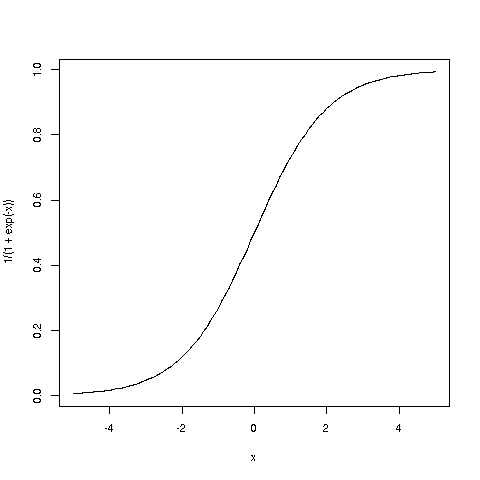
\includegraphics[width=3.05in]{Images/LogitCurve_gray.png}
}
\caption{Logistic function}
\label{logitcurve}
\end{figure}

Note the form of the curve, shown in Figure \ref{logitcurve}
The appeal of this model is clear at a glance:  First, the logistic function
produces a value in [0,1], as appropriate for modeling a probability.
Second, it is a monotone increasing function in each of the variables in
(\ref{logithighusage}), just as was the case in (\ref{bikelin}) for
predicting our numeric variable, {\bf reg}.  Other motivations for using
the logistic model will be discussed in Chapter \ref{chap:nonlin}.

R provides the {\bf glm()} (``generalized linear model'') function for
several nonlinear model families, including the logistic,\footnote{Often
called ``logit,'' by the way.} which is designated via {\bf family =
binomial}:

\begin{lstlisting}
> shar$highuse <- as.integer(shar$reg > 3500)
> glmout <- glm(highuse ~ 
     temp+temp2+workingday+clearday,
     data=shar,family=binomial)
> tmp <- coef(glmout) %*% c(1,0.525,0.525^2,0,1)
> 1/(1+exp(-tmp))
          [,1]
[1,] 0.1010449
\end{lstlisting}

So, our parametric model gives an almost identical result here to the
one arising from k-NN, about a 10\% probability of HighUsage.


\section{Crucial Advice: Don't Automate, Participate!}
\label{participate}

Data science should not be a ``spectator sport''; the methodology is
effective only if the users {\it participate}.  Avoid ceding the
decision making to the computer output.  For example:

\begin{itemize}

\item Statistical significance does not imply practical importance, and
conversely.

\item A model is just that --- just an approximation to reality,
hopefully useful but never exact.

\item Don't rely solely on variable selection algorithms to choose your
model (Chapter \ref{chap:dim}).

\item ``Read directions before use'' --- make sure you understand what a
method really does before employing it.

\end{itemize}

\section{Mathematical Complements}
\label{mcintro}

\subsection{Indicator Random Variables}
\label{indicvars}

A random variable $W$ is an indicator variable, if it is equal to 1 or
0, depending on whether a certain event $Q$ occurs or not.  Two simple
properties are very useful:

\begin{itemize}

\item $EW = P(Q)$

This follows from

\begin{equation}
EW = 1 \cdot P(Q) + 0 \cdot P(\textrm{not } Q) = P(Q)
\end{equation}

\item $Var(W) = P(Q) \cdot [1 - P(Q)]$

True because 

\begin{equation}
Var(W) = E(W^2) - (EW)^2 = E(W) - E(W^2) = EW (1 - EW)
\end{equation}

where the second equality stems from $W^2 = W$ (remember, $W$ is either
1 or 0).  Then use the first bullet above!

\end{itemize}


\subsection{Mean Squared Error of an Estimator}
\label{mse}

Say we are estimating some unknown population value $\theta$, using an
estimator $\widehat{\theta}$ based on our sample data.  Then a natural
measure of the accuracy of our estimator is the {\it Mean Squared
Error} (MSE),

\begin{equation}
E[(\widehat{\theta} - \theta)^2]
\end{equation}

This is the squared distance from our estimator to the true value, 
averaged over all possible samples.

Let's rewrite the quantity on which we are taking the expected value:

\begin{equation}
\label{msemess}
\left (
\widehat{\theta} - \theta
\right )^2 =
\left (
\widehat{\theta} - 
E\widehat{\theta} +
E\widehat{\theta} -
\theta
\right )^2
=
(\widehat{\theta} - E\widehat{\theta})^2 +
(E\widehat{\theta} - \theta)^2 + 
2 (\widehat{\theta} - E\widehat{\theta}) (E\widehat{\theta} - \theta)
\end{equation}

Look at the three terms on the far right of (\ref{msemess}).  The
expected value of the first is $Var(\widehat{\theta})$, by definition of
variance.

As to the second term, $E\widehat{\theta} - \theta$ is the {\it bias} of
$\widehat{\theta}$, the tendency of $\widehat{\theta}$ to over- or
underestimate $\theta$ over all possible samples.

What about the third term?  Note first that $E\widehat{\theta} - \theta$
is a constant, thus factoring out of the expectation.  But for what
remains,

\begin{equation}
E(\widehat{\theta} - E\widehat{\theta}) = 0
\end{equation}

Taking the expected value of both sides of (\ref{msemess}), and taking the
above remarks into account, we have

\begin{eqnarray}
\label{famousmse}
\textrm{MSE}(\widehat{\theta}) &=& Var(\widehat{\theta}) + 
(E\widehat{\theta} - \theta)^2 \\
&=& \textrm{variance} + \textrm{bias}^2
\end{eqnarray}

In other words:

\begin{quote}
The MSE of $\widehat{\theta}$ is equal to the 
variance of $\widehat{\theta}$ plus
squared bias of $\widehat{\theta}$.
\end{quote}

\subsection{$\mathbf{\mu}$(t) Minimizes Mean Squared Prediction Error}
\label{optimalmspe}

{\bf Claim:} {\it Consider all the functions f() with which we might
predict Y from X, i.e., $\widehat{Y} = f(X)$. The one that
minimizes mean squared prediction error, $E[(Y - f(X))^2]$, is
the regression function, $\mu(t) = E(Y ~|~ X = t).$}

(Note that the above involves population quantities, not samples.
Consider the quantity $E[(Y - f(X))^2]$, for instance.  It is the mean
squared prediction error (MSPE) over all $(X,Y)$ pairs in the
population.)

To derive this, first ask, for any (finite-variance) random variable
$W$, what number $c$ minimizes the quantity $E[(W - c)^2]$?  The
answer is $c = EW$.  To see this, 
write

\begin{equation}
\label{premse}
E[(W - c)^2] = E(W^2 - 2cW + c^2] = E(W^2) - 2c EW + c^2
\end{equation}

Setting to 0 the derivative of the right-hand side with respect to $c$,
we find that indeed, $c = EW$.

Now use the Law of Total Expectation (Section \ref{conditexpectprops}):

\begin{equation}
\textrm{MSPE} = E[(Y - f(X))^2] = 
E \left [
E( (Y - f(X))^2 | X)
\right ]
\end{equation}

In the inner expectation, $X$ is a constant, and from the statement
following (\ref{premse}) we know that the minimizing value of $f(X)$ is
``EW,'' in this case $E(Y | X)$, i.e.\ $\mu(X)$.  Since that minimizes
the inner expectation for any {\bf X}, the overall expectation is
minimized too.

\subsection{$\mu(t)$ Minimizes the Misclassification Rate}
\label{minerr}

We are concerned here with the classification context.  It shows that
if we know the population distribution --- we don't, but are going
through this exercise to guide our intuition --- the conditional mean
provides the optimal action in the classification context.

Remember, in this context, $\mu(t) = P(Y ~|~ X = t)$, i.e.\ the
conditional mean reduces to the conditional probability.  Now plug in
$X$ for $t$, and we have the following.

{\bf Claim:} {\it Consider all rules based on $X$ that produce a guess
$\widehat{Y}$, taking on values 0 and 1.  The one that minimizes the
overall misclassification rate $P(\widehat{Y} \neq Y)$ is}

\begin{equation}
\widehat{Y} = 
\begin{cases}
      1, & \textrm{ if } \mu(X) > 0.5 \\
      0, & \textrm{ if } \mu(X) \leq 0.5 
\end{cases}
\end{equation}

The claim is completely intuitive, almost trivial:  After observing $X$,
how should we guess $Y$?  If conditionally $Y$ has a greater than 50\%
chance of being 1, then guess it to be 1!

(Note:  In some settings, a ``false positive'' may be worse than a
``false negative,'' or {\it vice versa}.  The reader should ponder how
to modify the material here for such a situation.  We'll return to this
issue in Chapter \ref{chap:multiclass}.)

Think of this simple situation:  There is a biased coin, with
\textit{known} probability of heads p.  The coin will be tossed once,
and we are supposed to guess the outcome.

Let's name your guess $g$ (a nonrandom constant), and let C denote the
as-yet-unknown outcome of the toss (1 for heads, 0 for tails).  Then the
reader should check that, no matter whether we choose 0 or 1 for $g$,
the probability that we guess correctly is

\begin{eqnarray}
P(C = g) &=& P(C = 1) g + P(C = 0) (1-g) \\ 
&=& pg + (1-p)(1-g) \\
&=& [2 p - 1] g + 1 - p 
\label{twopq}
\end{eqnarray}

Now remember, $p$ is known.  How should we choose $g$, 0 or 1, in
order to maximize (\ref{twopq}), the probability that our guess is
correct?  Inspecting (\ref{twopq}) shows that maximizing that expression
will depend on whether $2p - 1$ is positive or negative, i.e., whether
$p > 0.5$ or not.  In the former case we should choose $g = 1$, while in
the latter case $g$ should be chosen to be 0.

The above reasoning gives us the very intuitive --- actually trivial,
when expressed in English --- result:

\begin{quote}
If the coin is biased toward heads, we should guess heads.  If the coin
is biased toward tails, we should guess tails.
\end{quote}
 
Now to show the original claim, we use The Law of Total Expectation.
This will be discussed in detail in Section \ref{conditexpectprops},
but for now, it says this:

\begin{equation}
E(V) = E[E(V|U)]
\end{equation}

i.e.\ the expected value of a conditional random variable is the
unconditional expectation.  In the case where $V$ is an indicator random
variable, the above reduces to

\begin{equation}
\label{peqepgivu}
P(A) = E[P(A ~|~ U)] 
\end{equation}

Returning to our original claim, write

\begin{equation}
P(\widehat{Y} = Y) = 
E \left [
P(\widehat{Y} = Y ~|~ X) 
\right ]
\end{equation}

In that inner probability, ``p'' is 

\begin{equation}
P(Y = 1 ~|~ X) = \mu(X)
\end{equation}

which completes the proof.

% \subsection{Kernel-Based Nonparametric Estimation of \\ Regression
% Functions}
% \label{kernelbased}
% 
% In Section \ref{knnmethod}, we introduced the k-Nearest Neighbor method
% for nonparametric estimation of regression functions.  Another popular
% approach is the {\it kernel method}, which we will discuss here.
% 
% Say $Y$ is human weight, and $X$ is height, so we are estimating the
% regression of weight against height.  Suppose we have a sample of 1000
% people with known weights and heights, and wish to estimate $\mu(70)$.
% How might we compute our estimate $\widehat{\mu}(70)$?
% 
% With k-NN, say setting $k = 25$, we would find the 25 people in our
% sample whose heights are closest to 70, and set $\widehat{\mu}(70)$ to
% the average weight among those 25 people.  
% 
% So, the number of people we use to compute $\widehat{\mu}(70)$ is
% \textit{fixed}, at 25, while the largest distance away from 70 among
% those people is \textit{random}:  The 1000 people are assumed to be a
% random sample from whatever target population we have.
% 
% With the kernel method, it's exactly the opposite:  The number of people
% used to compute $\widehat{\mu}(70)$ will be \textit{random}, but the
% largest distance from 70 among them will be \textit{fixed}.
% 
% For example, we might decide to base $\widehat{\mu}(70)$ on whichever
% people have heights within, say, 2.2 inches of 70.0.  The 2.2 is a fixed
% quantity, but the number of people who fall into that (67.8,72.2) range
% will be random.
% 
% Now, to explain the word {\it kernel}, first write the above as
% 
% \begin{equation}
% \label{kerneldef}
% \widehat{\mu}(70) = 
% \frac
% { \sum_{i=1}^n k(X_i,70) ~ Y_i }
% { \sum_{i=1}^n k(X_i,70) }
% \end{equation}
% 
% where $k()$ is the kernel, in this case
% 
% \begin{equation}
% \label{unifkern}
% k(x,t) = 
% \begin{cases}
%       1, & \textrm{ if } |x-t| \leq 2.2 \\
%       0, & \textrm{ if } |x-t| > 2.2
% \end{cases}
% \end{equation}
% 
% Though somewhat imposing, this formulation does work. Since $k()$ takes
% on only the values 1 and 0, the numerator in (\ref{kerneldef}) is simply
% the sum of the weights of the people with heights within 2.2 of 70,
% while the denominator is the number of such people --- exactly what we
% want.
% 
% But the point is that we can use kernels other than (\ref{unifkern}).
% In the above analysis, we are giving equal weighting to all the people
% in the given interval, whether their heights are very near 70.0 or near
% 67.8 or 72.2.  It would seem more accurate to weight the cases near 70.0
% more heavily.  
% 
% One choice of kernel that would do this is
% 
% \begin{equation}
% \label{unifkern}
% k(x,t) = 
% \begin{cases}
%       2.2 - |x-t|, & \textrm{ if } |x-t| \leq 2.2 \\
%       0, & \textrm{ if } |x-t| > 2.2
% \end{cases}
% \end{equation}
% 
% We spoke earlier of the fact that the number of nearest neighbors in
% k-NN is a {\it tuning parameter}, meaning a value that must be chosen by
% the user.  With the kernel method above, the 2.2 is also a tuning
% parameter, called the {\it bandwidth}.  As noted earlier, the values of
% tuning parameters are often chosen via cross-validation.
% 
% The kernel function {\bf k()} (not related to the 'k' in 'k-NN,' of
% course) can be thought of as a tuning parameter.  But typically the
% choice of kernel is less important than the cboice of the bandwidth.
% 
% \subsection{General Nonparametric Regression}
% 
% Besides k-NN and kernel estimation, another common nonparametric method
% is {\it spline smoothing}.  Though we will use k-NN extensively in this
% book, we will not present a detailed analysis of k-NN, kernel and spline
% techniques.  See \cite{simonoff} for more.  The methods in Chapter
% \ref{chap:partitions} of the present book also can be considered
% nonparametric.

\subsection{Some Properties of Conditional Expectation}
\label{conditexpectprops}

Since the regression function is defined as a conditional expected
value, as in (\ref{regdef}), for mathematical analysis we'll need some
properties. First, a definition.

\subsubsection{Conditional Expectation As a Random \\ Variable}

For any random variables $U$ and $V$ with defined expectation, either of
which could be vector-valued, define a new random variable $W$, as
follows.  First note that the conditional expectation of $V$ given $U =
t$ is a function of $t$,

\begin{equation}
\label{mutagain}
\mu(t) = E(V ~|~ U = t)
\end{equation}

This is an ordinary function, just like, say, $\sqrt{t}$.  But we can
turn that ordinary function into a random variable by plugging in a
random variable, say $Q$, for $t$:  $R = \sqrt{Q}$ is a random variable.
Thinking along these lines, we define the {\it random variable} version
of conditional expectation accordingly.  In the {\it function} $\mu(t)$
in (\ref{mutagain}), we plug in $U$ for $t$:

\begin{equation}
W = E(V | U) = \mu(U)
\end{equation}

This $W$ is a random variable.  As a simple example, say we choose a
number $U$ at random from the numbers 1 through 5.  We then randomly
choose a second number $V$, from the numbers 1 through $U$.  Then

\begin{equation}
\mu(t) = E(V ~|~ U = t) = \frac{1+t}{2}
\end{equation}

We now form a new random variable $W = (1+U)/2$.

And, since $W$ is a random variable, we can talk of {\it its} expected
value, which turns out to be an elegant result:

\subsubsection{The Law of Total Expectation}
\label{totexpsec}

A property of conditional expected value, proven in many undergraduate
probability texts, is

\begin{equation}
\label{totexp}
E(V) = EW = E[E(V ~|~ U)]
\end{equation}

The foreboding appearance of this equation belies the fact that it is
actually quite intuitive, as follows.  Say you want to compute the mean
height of all people in the U.S., and you already have available the
mean heights in each of the 50 states.  You cannot simply take the
straight average of those state mean heights, because you need to give
more weight to the more populous states.  In other words, the national
mean height is a {\it weighted} average of the state means, with the
weight for each state being its proportion of the national
population.  

In (\ref{totexp}), this corresponds to having $V$ as height and $U$ as
state.  State coding is an integer-valued random variable, ranging 
from 1 to 50, so we have

\begin{eqnarray}
EV &=& E[E(V ~|~ U)] \\
&=& EW \\
&=& \sum_{i=1}^{50} P(U = i) ~ E(V ~|~ U = i)
\end{eqnarray}

The left-hand side, $EV$, is the overall mean height in the nation;
$E(V ~|~ U = i)$ is the mean height in state $i$; and the weights in the
weighted average are the proportions of the national population in each
state, $P(U = i)$.

% The above is for population quantities.  It holds on the sample level
% too.
% 
% \iffalse
% library(freqparcoord)
% data(mlb)
% lm(mlb$Weight ~ mlb$Height + mlb$Age)
% \fi 

Not only can we look at the mean of $W$, but also its variance.  By
using the various familiar properties of mean and variance, one can
derive a similar relation for variance: 

\subsubsection{Law of Total Variance}

For scalar $V$,

\begin{equation}
\label{totvar}
Var(V) = E[Var(V|U)] + Var[E(V|U)]
\end{equation}

One might initially guess that we only need the first term.  To obtain
the national variance in height, we would take the weighted average of
the state variances.  But this would not take into account that the mean
heights vary from state to state, thus also contributing to the national
variance in height, hence the second term.

This is proven in Section \ref{itsaprojection}.

\subsubsection{Tower Property}
\label{tower}

Now consider conditioning on two variables, say $U_1$ and $U_2$.  One
can show that

\begin{equation}
E 
\left [
E(V | U_1, U_2) ~|~ U_1
\right ]
= E(V ~|~ U_1)
\end{equation}

Here is an intuitive interpretation of that in the height example above.
Take $V$, $U_1$ and $U_2$ to be height, state and gender, respectively,
so that $E(V | U_1, U_2)$ is the mean height of all people in a certain
state and of a certain gender.  If we then take the mean of all these
values for a certain state --- i.e.\ take the average of the two
gender-specific means in the state --- we get the mean height in the
state without regard to gender.

Again, note that we take the straight average of the two gender-specific
means, because the two genders have equal proportions.  If, say, $U_2$
were race instead of gender, we would need to compute a {\it weighted}
average of the race-specific means, with the weights being the
proportions of the various races in the given state.

This is proven in Section \ref{projecttwice}.

\subsubsection{Geometric View}
\label{geomview}

There is an elegant way to view all of this in terms of abstract vector
spaces --- (\ref{totexp}) becomes the Pythagorean Theorem! ---
which we will address later in Mathematical Complements
Sections \ref{geom} and \ref{projecttwice}.

\section{Computational Complements}

\subsection{CRAN Packages}
\label{cranpkgs}

There are thousands of useful contributed R packages available on
CRAN, the Comprehensive R Archive Network,
\textit{https://cran.r-project.org}.  The easiest way to install them is
from R's interactive mode, e.g.

\begin{lstlisting}
> install.packages('freqparcoord','~/R')
\end{lstlisting}

Here I have instructed R to download the {\bf freqparcoord}
package, installing it in \lstinline{~/R}, the directory where I like to
store my packages.  

(If you are using RStudio or some other indirect interface to R, all
this can be done from a menu, rather than using {\bf
installing.packages}.)

Official R parlance is {\it package}, not {\it library}, even though
ironically one loads a package using the {\bf library()} function!  For
instance,

\begin{lstlisting}
> library(freqparcoord)
\end{lstlisting}

One can learn about the package in various ways.  After loading it, for
instance, you can list its objects, such as

\begin{lstlisting}
> ls('package:freqparcoord')
[1] "freqparcoord" "knndens"      "knnreg"       
"posjitter"     "regdiag"     
[6] "regdiagbas"   "rmixmvnorm"   "smoothz"      
"smoothzpred" 
\end{lstlisting}

where we see objects (functions here) {\bf knndens()} and so on.  There
is the {\bf help()} function, e.g.

\begin{lstlisting}
> help(package=freqparcoord) 

Information on package ‘freqparcoord’

Description:

Package:       freqparcoord
Version:       1.1.0
Author:        Norm Matloff <normmatloff@gmail.com>  
               and Yingkang Xie 
               <yingkang.xie@gmail.com>
Maintainer:    Norm Matloff <normmatloff@gmail.com>
...
\end{lstlisting}

Some packages have {\it vignettes}, extended tutorials.  Type

\begin{lstlisting}
> vignette()
\end{lstlisting}

to see what's available.

\subsection{The Function {\bf tapply()} and Its Cousins}
\label{tapply}

In Section \ref{firstest} we had occasion to use R's {\tt tapply()}, a
highly useful feature of the language.  To explain it, let's start with
useful function, {\bf split()}.

Consider this tiny data frame:

\begin{lstlisting}
> x
  gender height
  1      m     66
  2      f     67
  3      m     72
  4      f     63
\end{lstlisting}

Now let's split by gender:

\begin{lstlisting}
> xs <- split(x,x$gender)
> xs
$f
  gender height
2      f     67
4      f     63
5      f     63

$m
  gender height
1      m     66
3      m     72
\end{lstlisting}

Note the types of the objects: 

\begin{itemize}

\item {\bf xs} is an R list

\item {\bf xs\$f} and {\bf xs\$m} are data frames, the male and female
subsets of {\bf x}

\end{itemize}

We {\it could} then find the mean heights for each gender this way:

\begin{lstlisting}
> mean(xs$f$height)
[1] 64.33333
> mean(xs$m$height)
[1] 69
\end{lstlisting}

But with {\bf tapply()}, we can combine the two operations:

\begin{lstlisting}
> tapply(x$height,x$gender,mean)
       f        m 
64.33333 69.00000 
\end{lstlisting}

The first argument of {\tt tapply()} must be a vector, but the function
that is applied can be vector-valued.  Say we want to find not only the
mean but also the standard deviation.  We can do this:

\begin{lstlisting}
> tapply(x$height,x$gender,function(w) c(mean(w),sd(w)))
$f
[1] 64.333333  2.309401

$m
[1] 69.000000  4.242641
\end{lstlisting}

Here our function, which we defined ``on the spot,'' within our call to
{\bf tapply()}, produces a vector of two components.  We asked {\bf
tapply()} to call that function on our vector of heights, doing so
separately for each gender.

As noted in the title of this section, {\bf tapply()} has ``cousins.''
Here is a brief overview of some of them:

\begin{lstlisting}
# form a matrix by binding the rows (1,2) and (3,4)
> m <- rbind(1:2,3:4)
> m
     [,1] [,2]
[1,]    1    2
[2,]    3    4
# apply the sum() function to each row
> apply(m,1,sum)
[1] 3 7
# apply the sum() function to each column
> apply(m,2,sum)
[1] 4 6
\end{lstlisting}

\begin{lstlisting}
> l <- list(a = c(3,8), b = 12)
> l
$a
[1] 3 8
$b
[1] 12
# apply sum() to each element of the list, 
# forming a new list
> lapply(l,sum)
$a
[1] 11
$b
[1] 12
# do the same, but try to reduce the result 
# to a vector
> sapply(l,sum)
 a  b 
11 12 
\end{lstlisting}

\subsection{The Innards of the k-NN Code}

Here are simplified versions of the code:

\begin{lstlisting}
preprocessx <- function(x,kmax,xval=FALSE) {
   result$x <- x
   tmp <- FNN::get.knnx(data=x, query=x, k=kmax+xval)
   nni <- tmp$nn.index
   result$idxs <- nni[,(1+xval):ncol(nni)]
   result$xval <- xval
   result$kmax <- kmax
   class(result) <- 'preknn'
   result
}
\end{lstlisting}

The code is essentially just a wrapper for calls to the {\bf FNN}
package on CRAN, which does nearest-neighbor computation.

\begin{lstlisting}
knnest <- function(y,xdata,k,nearf=meany)
{
   idxs <- xdata$idxs
   idx <- idxs [,1:k]
   # set idxrows[[i]] to row i of idx, the indices of
   # the neighbors of the i-th observation
   idxrows <- matrixtolist(1,idx)
   # now do the kNN smoothing
   # first, form the neighborhoods
   x <- xdata$x
   xy <- cbind(x,y)
   nycol <- ncol(y)  # how many cols in xy are y?
   # ftn to form one neighborhood (x and y vals)
   form1nbhd <-  function(idxrow) xy[idxrow,]
   # now form all the neighborhoods
   nearxy <- 
      lapply(idxrows,function(idxrow) xy[idxrow,])
   # now nearxy[[i]] is the rows of x corresponding to
   # neighbors of x[i,], together with the associated 
   # Y values

   # now find the estimated regression function values 
   # at each point in the training set
   regest <- sapply(1:nrow(x),
      function(i) nearf(x[i,],nearxy[[i]]))
   regest <- 
      if (nycol > 1) t(regest) else as.matrix(regest)
   xdata$regest <- regest
   xdata$nycol <- nycol
   xdata$y <- y
   xdata$k <- k
   class(xdata) <- 'knn'
   xdata
}

\end{lstlisting}

\subsection{Function Dispatch}
\label{dispatch}

The return value from a call to {\bf lm()} is an object of R's S3 class
structure; the class, not surprisingly, is named {\bf `lm'}.  It turns
out that the functions {\bf coef()} and {\bf vcov()} mentioned in this
chapter are actually related to this class, as follows.

Recall our usage, on the baseball player data:

\begin{lstlisting}
> lmout <- lm(mlb$Weight ~ mlb$Height)
> coef(lmout) %*% c(1,72)
         [,1]
[1,] 193.2666
\end{lstlisting}

The call to {\bf coef} extracted the vector of estimated regression
coefficents (which we also could have obtained as {\bf
lmout\$coefficents}).  But here is what happened behind the scenes:

The R function {\bf coef()} is a {\it generic function}, which means
it's just a placeholder, not a ``real'' function.  When we call it, the
R interpreter says, 

\begin{quote}

This is a generic function, so I need to relay this call to the one
associated with this class, {\bf `lm'}.  That means I need to check
whether we have a function {\bf coef.lm()}.  Oh, yes we do, so let's
call that.

\end{quote}

That relaying action is referred to in R terminology as the original
call being {\it dispatched} to {\bf coef.lm()}.

This is a nice convenience.  Consider another generic R function, {\bf
plot()}.  No matter what object we are working with, the odds are that
some kind of plotting function has been written for it.  We can just
call {\bf plot()} on the given object, and leave it to R to find the
proper call.  (This includes the {\bf `lm'} class; try it on our {\bf
lmout} above!)

Similarly, there are a number of R classes on which {\bf coef()} is
defined, and the same is true for {\bf vcov()}.

One generic function we will use quite often, and indeed have already
used in this chapter, is {\bf summary()}.  As its name implies, it
summarizes (what the function's author believes) are the most important
characteristics of the object.  So, when this generic function is called
on an {\bf `lm'} object, the call is dispatched to {\bf summary.lm()},
yielding estimated coefficients, standard errors and so on.

Another generic function to be used often here is {\bf predict()}, from
Section \ref{predictfun}.  In the example there, {\bf lmout} was of
class {\bf `lm'}, so the call to {\bf predict()} was dispatched to {\bf
predict.lm()}.

\section{Centering and Scaling}
\label{centerscale}

It is common in many statistical methods to {\it center and scale} the
data.  Here we subtract from each variable the sample mean of that
variable.  This process is called {\it centering}.  Typically one also
{\it scales} each predictor, i.e.\ divides each predictor by its sample
standard deviation.  Now all variables will have mean 0 and standard
deviation 1.

It is clear that this is very useful for k-NN regression.
Consider the example later in this chapter involving Census data.
Without at least scaling, variables that are very large, such as income,
would dominate the nearest-neighbor computations, and small but
important variables such as age would essentially be ignored.  The 
{\bf knnest()} function that we will be using does do centering and
scaling as preprocessing for the predictor variables.

In a parametric setting such as linear models, centering and scaling has
the goal of reducing numerical roundoff error.  

In R, the centering/scaling operation is done with the {\bf scale()}
function.  In order to be able to reverse the process later, the means
and standard deviations are recorded as R {\it attributes}:

\begin{lstlisting}
> m <- rbind(1:2,3:4)
> m
     [,1] [,2]
[1,]    1    2
[2,]    3    4
> m1 <- scale(m)
> m1
           [,1]       [,2]
[1,] -0.7071068 -0.7071068
[2,]  0.7071068  0.7071068
attr(,"scaled:center")
[1] 2 3
attr(,"scaled:scale")
[1] 1.414214 1.414214
> attr(m1,'scaled:center')
[1] 2 3
\end{lstlisting}

\startproblemset

{\bf Data problems:}

\oneproblem
\label{randomxval}
In Section \ref{applyingxval}, the reader was reminded that the results
of a cross-validation are random, due to the random partitioning into
training and test sets.  Try doing several runs of the linear and k-NN
code in that section, comparing results.

\oneproblem
Extend (\ref{pefem}) to include interaction terms for age and gender,
and age$^{2}$ and gender.  Run the new model, and find the estimated
effect of being female, for a 32-year-old person with a Master's degree.

\oneproblem
Consider the {\bf bodyfat} data mentioned in Section \ref{bodyfat}.  Use
{\bf lm()} to form a prediction equation for {\bf density} from the
other variables (skipping the first three), and comment on whether use
of indirect methods in this way seems feasible.

\oneproblem
In Section \ref{totexpsec}, we gave this intuitive explanation:

\begin{quote}

In other words, the national mean height is a {\it weighted} average of
the state means, with the weight for each state being its proportion of
the national population.   Replace state by gender in the following.

\end{quote}

\begin{itemize}

\item [(a)]  Write English prose that relates the overall mean height of
people and the gender-specific mean heights.

\item [(b)]  Write English prose that relates the overall proportion of
people taller than 70 inches to the gender-specific proportions.

\end{itemize}

{\bf Mini-CRAN and other computational problems:}

\oneproblem
In Section \ref{xval}, we used R's negative-index capability to form 
the training/test set partitioning.  Show how we could use the R 
function {\bf setdiff()} to do this as an alternate approach.  

\oneproblem
We saw in this chapter, e.g., in Figure \ref{addedabline}, how R's 
{\bf abline()} function can be used to add a straight line to a plot.
What about adding a quadratic function?

\begin{itemize}

\item [(a)]
Write an R function with call form

\begin{lstlisting}
abccurve(coef,xint)
\end{lstlisting}

where {\bf coef} is a vector of the coeficients $a$, $b$ and $c$ in the
polynomial

\begin{equation}
a + b t + c t^2
\end{equation}

and {\bf xint} is a 2-element vector that gives the range of the
horizontal axis for $t$.  The function superimposes the quadratic curve
onto the existing graph.  Hint:  Use R's {\bf curve()} function.

\item [(b)]
Fit a quadratic model to the click-through data, and use your {\bf
abccurve()} function on the scatter plot for that data.

\end{itemize}

{\bf Math problems:}

\oneproblem
Suppose the joint density of $(X,Y)$ is $3s^2 e^{-st}, ~ 1 < s < 2, 0 < t
< \infty$.  Find the regression function $\mu(s) = E(Y | X = s)$.

\oneproblem
For $(X,Y)$ in the notation of Section \ref{optimalmspe}, show that the 
predicted value $\mu(X)$ and the predicton error $Y - \mu(X)$ are
uncorrelated.

\oneproblem
Suppose $X$ is a scalar random variable with density $g$.  We are
interested in the nearest neighbors to a point $t$, based on a random
sample $X_1,...,X_n$ from $g$.  Find $L_k$, the cumulative
distribution function of the distance of the $k^{th}$-nearest neighbor
to $t$.
% The kth will be at most c distant iff at least k are within c of t.

